\chapter{HeROfake}

\section{Introduction}

\begin{table*}[t]
    \centering
        \caption{State of the Art work on autoscaling platforms}
        \begin{tabular}{lccccccc}
            \toprule
            & Serverless & Target cloud platform     & SLA & Hardware heterogeneity & Resources usage & Energy consumption & Cost-aware \\
            \cmidrule(lr){2-2}\cmidrule(lr){3-3}\cmidrule(lr){4-4}\cmidrule(lr){5-5}\cmidrule(lr){6-6}\cmidrule(lr){7-7}\cmidrule(lr){8-8}
            Swayam~\cite{gujaratiSwayamDistributedAutoscaling2017}        & \xmark         & Private (Azure, in-house) & \cmark& \xmark                     & \cmark            & \xmark                 & \xmark         \\
            Pigeon~\cite{lingPigeonDynamicEfficient2019}                  & \cmark       & Private                   & \xmark  & \cmark                   & \cmark            & \xmark                 & \xmark         \\
            MArk~\cite{zhangMArkExploitingCloud}                          & \xmark         & Public (AWS)              & \cmark& \cmark                   & \cmark            & \xmark                 & \cmark       \\
            ENSURE~\cite{sureshENSUREEfficientScheduling2020}             & \cmark       & Private                   & \xmark  & \xmark                     & \cmark            & \xmark                 & \cmark       \\
            Mampage et al.~\cite{mampageDeadlineawareDynamicResource2021} & \cmark       & Private                   & \cmark& \xmark                     & \cmark            & \xmark                 & \cmark       \\
            Atoll~\cite{singhviAtollScalableLowLatency2021}               & \cmark       & Private                   & \cmark& \xmark                     & \xmark              & \xmark                 & \xmark         \\
            INFless~\cite{yangINFlessNativeServerless2022}                & \cmark       & Private                   & \cmark& \xmark                     & \cmark            & \xmark                 & \cmark       \\
            SMIF~\cite{choSLADrivenMLInference}                           & \cmark       & Private                   & \cmark& \cmark                   & \cmark            & \xmark                 & \xmark         \\
            Target solution                                                & \cmark       & Private                   & \cmark& \cmark                   & \cmark            & \cmark               & \cmark       \\ \bottomrule
        \end{tabular}%
    \label{table:herofake-sota}
\end{table*}

%\subsection{The serverless service model}

\textbf{Serverless model}. Serverless can be understood as both a programming model, called Function as a Service (FaaS), and a deployment model for the cloud. In such a model, developers design their applications as a composition of stateless functions which execution is event-driven~\cite{SchleierSmith2021WhatSC}. 
Serverless services free tenants from complex resource reservation as they are designed to handle on-demand scaling requirements. % and address fluctuations in demand, therefore freeing tenants from the burden of having to define explicit scaling strategies.

In the FaaS model, providers only bill customers according to their actual resources usage~\cite{jonasCloudProgrammingSimplified2019}. They are fully responsible for deploying intelligent resource management and multiplexing at a finer granularity to optimize Quality of Service (QoS) metrics such as response time, energy consumption, etc. %while enabling providers to share physical resources at a higher degree of multiplexing, thus achieving better efficiency.

%\subsection{Deepfake and serverless}

\textbf{Deepfake detection and serverless}. The work presented in this paper was part of a project (at the b{\textless\textgreater}com research institute \footnote{\href{https://b-com.com/en}{https://b-com.com/en}}) aimed at deploying an energy efficient deepfake detection service in a heterogeneous cloud. Deepfakes are synthetic images, videos or speeches, digitally created to mimic an existing person so as to mislead viewers. Deepfake detection consists in training a Convolutional Neural Network (CNN) to detect patterns of inconsistencies that are introduced in the creation process.

The functions used by our deepfake application satisfy three main characteristics for suitable serverless workloads~\cite{cncf2018whitepaper}: their execution can be made parallel (several independent images and videos), they are stateless (pure transformation on input data) and event-driven (launched after data upload).

%On the one hand, deepfake detection using convolutional neural networks (CNNs) is a task that can take advantage of concurrency by running multiple convolutions in parallel and/or by handling different images on multiple threads. These tasks are essentially stateless, as they apply a pure transformation on input data -- taking an image as input and returning a boolean value as output. Such an application is event-driven, with computation starting following the upload of an input image. These are three main characteristics of suitable serverless workloads~\cite{cncf2018whitepaper}.

%On the other hand, the hardware resources needed to run that application at scale would be numerous and costly: being able to dynamically scale the resources in and out following demand would provide important savings to the client, and allow the provider to accept more clients on the same number of nodes.

%Therefore, we argue that the serverless service model is a perfect fit for cost-effective, on-demand inference using CNNs.

%\subsection{Hardware heterogeneity in the cloud}

\textbf{Hardware heterogeneity in the cloud}. Cloud infrastructures are more and more heterogeneous to fit the needs of data-intensive applications such as machine learning model training or big data analytics~\cite{reissHeterogeneityDynamicityClouds}. However, specialized processors and GPUs are yet to be made available to customers in serverless offerings~\cite{khandelwalTaureauDeconstructingServerless2020}. Hardware acceleration should be decided by the provider on a per-application or per-request basis.

State-of-the-art work shows that using such hardware in a cloud setting provides substantial gains in execution time and energy consumption~\cite{10.1145/3369583.3392679, 9195730}. However, reference orchestrators such as Kubernetes with Knative or OpenWhisk lack the support for dynamic allocation of such hardware. %capability to automatically and efficiently benefit from heterogeneous clouds. %deploy applications to nodes that provide relevant hardware to accelerate execution.

%with demand in GPUs and specialized processing cores driven by increasingly data-intensive computations with tasks such as machine learning model training or big data analytics. These heterogeneous computing units are yet to be made available to customers in serverless offerings~\cite{khandelwalTaureauDeconstructingServerless2020}. Hardware acceleration should be decided by the provider on a per-application or per-request basis.

%\subsection{Performance challenges}

\textbf{Performance challenge for serverless deployment}. Due to the transient nature of unreserved FaaS resources, latency, throughput and continuity of service are hard to guarantee~\cite{vaneykSPECRGCloud2018, dartoisCuckooOpportunisticMapReduce2019}. When applications do not receive incoming requests, function sandboxes are destroyed instead of being kept in an idle state. Then, when a new request arrives, the provider has to (re)allocate resources and initialize functions to deploy new sandboxes: this is called a cold start. Cold start times are very penalizing for the application performance, they may even dominate the total execution times~\cite{mullerLambadaInteractiveData2020}.

Furthermore, in current commercial serverless offerings, Service-Level Agreements (SLAs) are usually limited to automated retries (restarts) on failure, and FaaS providers generally limit the execution time of serverless functions to a few minutes. The absence of QoS guarantees in commercial serverless offerings prevents them from being more widely used~\cite{buyyaSLAorientedResourceProvisioning2011}.

%\subsection{Problem statement}

\textbf{Problem statement -- putting it all together}. The problem we try to solve in this paper is to determine how to automatically and reactively scale heterogeneous hardware resources in a cloud in adequacy with the application's load and the users' QoS requirements, while keeping the cost in resources and energy as low as possible for the provider. We consider a deepfake detection application as a case study in our work.

%Rather than reserving nodes in their infrastructure for an interactive application which load is unpredictable~\cite{shahradServerlessWildCharacterizing}, the provider can rely on a serverless platform for cost efficiency. The platform will automatically and reactively scale hardware resources in adequacy with the application's load.

%To be efficient in terms of cost and energy consumption, an autoscaling platform should be able to rightsize the allocated resources in a serverless cloud infrastructure, while being responsive enough to accommodate workload changes without impacting end users with spikes in latency. In order to meet per-user QoS requirements, it should take into account the characteristics of heterogeneous hardware resources, and SLAs should be negotiated on a per-request basis rather than on a per-function basis.

%\subsection{State of the Art}
\textbf{State-of-the-art}. Previous studies have explored the need for an autoscaling platform that supports short-running tasks comprised in applications such as Machine Learning as a Service. Table~\ref{table:herofake-sota} summarizes how these solutions differ from the target platform we are trying to achieve, and Section~\ref{section:herofake-sota} provides further details. While many have established the need for on-demand acceleration as a solution to guaranteeing function response time, none have measured the impact of leveraging heterogeneous resources on dynamic energy consumption. Furthermore, previous studies consider task consolidation as a means to free resources for further computations -- we argue that such techniques open possibilities for the service provider to apply power saving policies in private clouds. Finally, as serverless platforms are general purpose and designed to be highly configurable, our target solution should be cost-aware to allow the provider to make configuration choices pertaining to their own objectives.

%\subsection{Our contribution}
%\jb{à revoir ... j'ai l'impression que ça ne décrit pas correctement la contrib}

\textbf{Our contribution}. We argue that opportunistically taking advantage of hardware accelerators (GPUs and FPGAs) to schedule deepfake detection tasks may allow cloud providers to guarantee serverless tasks response time and achieve SLA while reducing resource usage and energy consumption.

In this paper, we propose a full framework to deploy a deepfake detection application on a serverless cloud. This framework comprises an offline and an online phase. The \textbf{offline phase} is used to characterize the performance and energy behavior of the deployed heterogeneous hardware platforms. The \textbf{online phase} consists of an autoscaling platform and a scheduling strategy that make efficient use of (characterized) heterogeneous hardware resources to achieve per-request SLAs while reducing the energy consumption of the platform. 

%\begin{itemize}
%    \item platform-level sandbox caching to minimize cold start delays \jb{tu fais des choses explicite sur le sujet ?};
%    \item QoS requirements at the granularity of a task to avoid penalties.
%\end{itemize}

%This is made possible by implementing these tasks for different hardware architectures, and measuring their performance and energy consumption ahead of scheduling (see Section~\ref{characterization}). \jb{tu insistes sur les inputs, plutôt que sur les techniques }

For this case study, we devised a simulation environment\footnote{The simulator repository will be made publicly available.} that models the infrastructure for a deepfake detection application, run by the provider as a Software as a Service using a serverless infrastructure.   %\vl{oui, il faut que je fasse la demande de divulgation de propriété intellectuelle à bcom - montre moi le mail d'abord, il faut insister sur l'utilité de la mise en ligne}

%By factoring in workload characterization (see Section~\ref{characterization}) in order to predict tasks performances on different execution platforms, we are able to avoid pre-allocating resources while keeping the frequency of cold starts under 0.02\% of function startups.

\textbf{Some performance figures}. With our allocation and scheduling policy, we were able to handle 50000 tasks in the same makespan as Knative with less than 36\% QoS penalties. Our framework reduces energy consumption for the execution of tasks by almost 35\%, and provides the opportunity for the provider to further reduce static power consumption by consolidating tasks on less than 29\% of the available nodes.

The paper is organized as follows: in a first section, we describe the overall platform model for the project. Then, we describe the execution platform and workload characterization phase. In Section III we describe the challenges of serverless resource orchestration, our task model and the orchestrator's allocation and scheduling policies. Section IV presents our evaluation methodology and a discussion of the experimental results. Section V gives details regarding state-of-the-art work on autoscaling platforms. Finally, we conclude with some perspectives for future work.

\section{Deploying Deepfake Detection Tasks in Serverless Cloud}

\begin{figure*}[t]
\centering
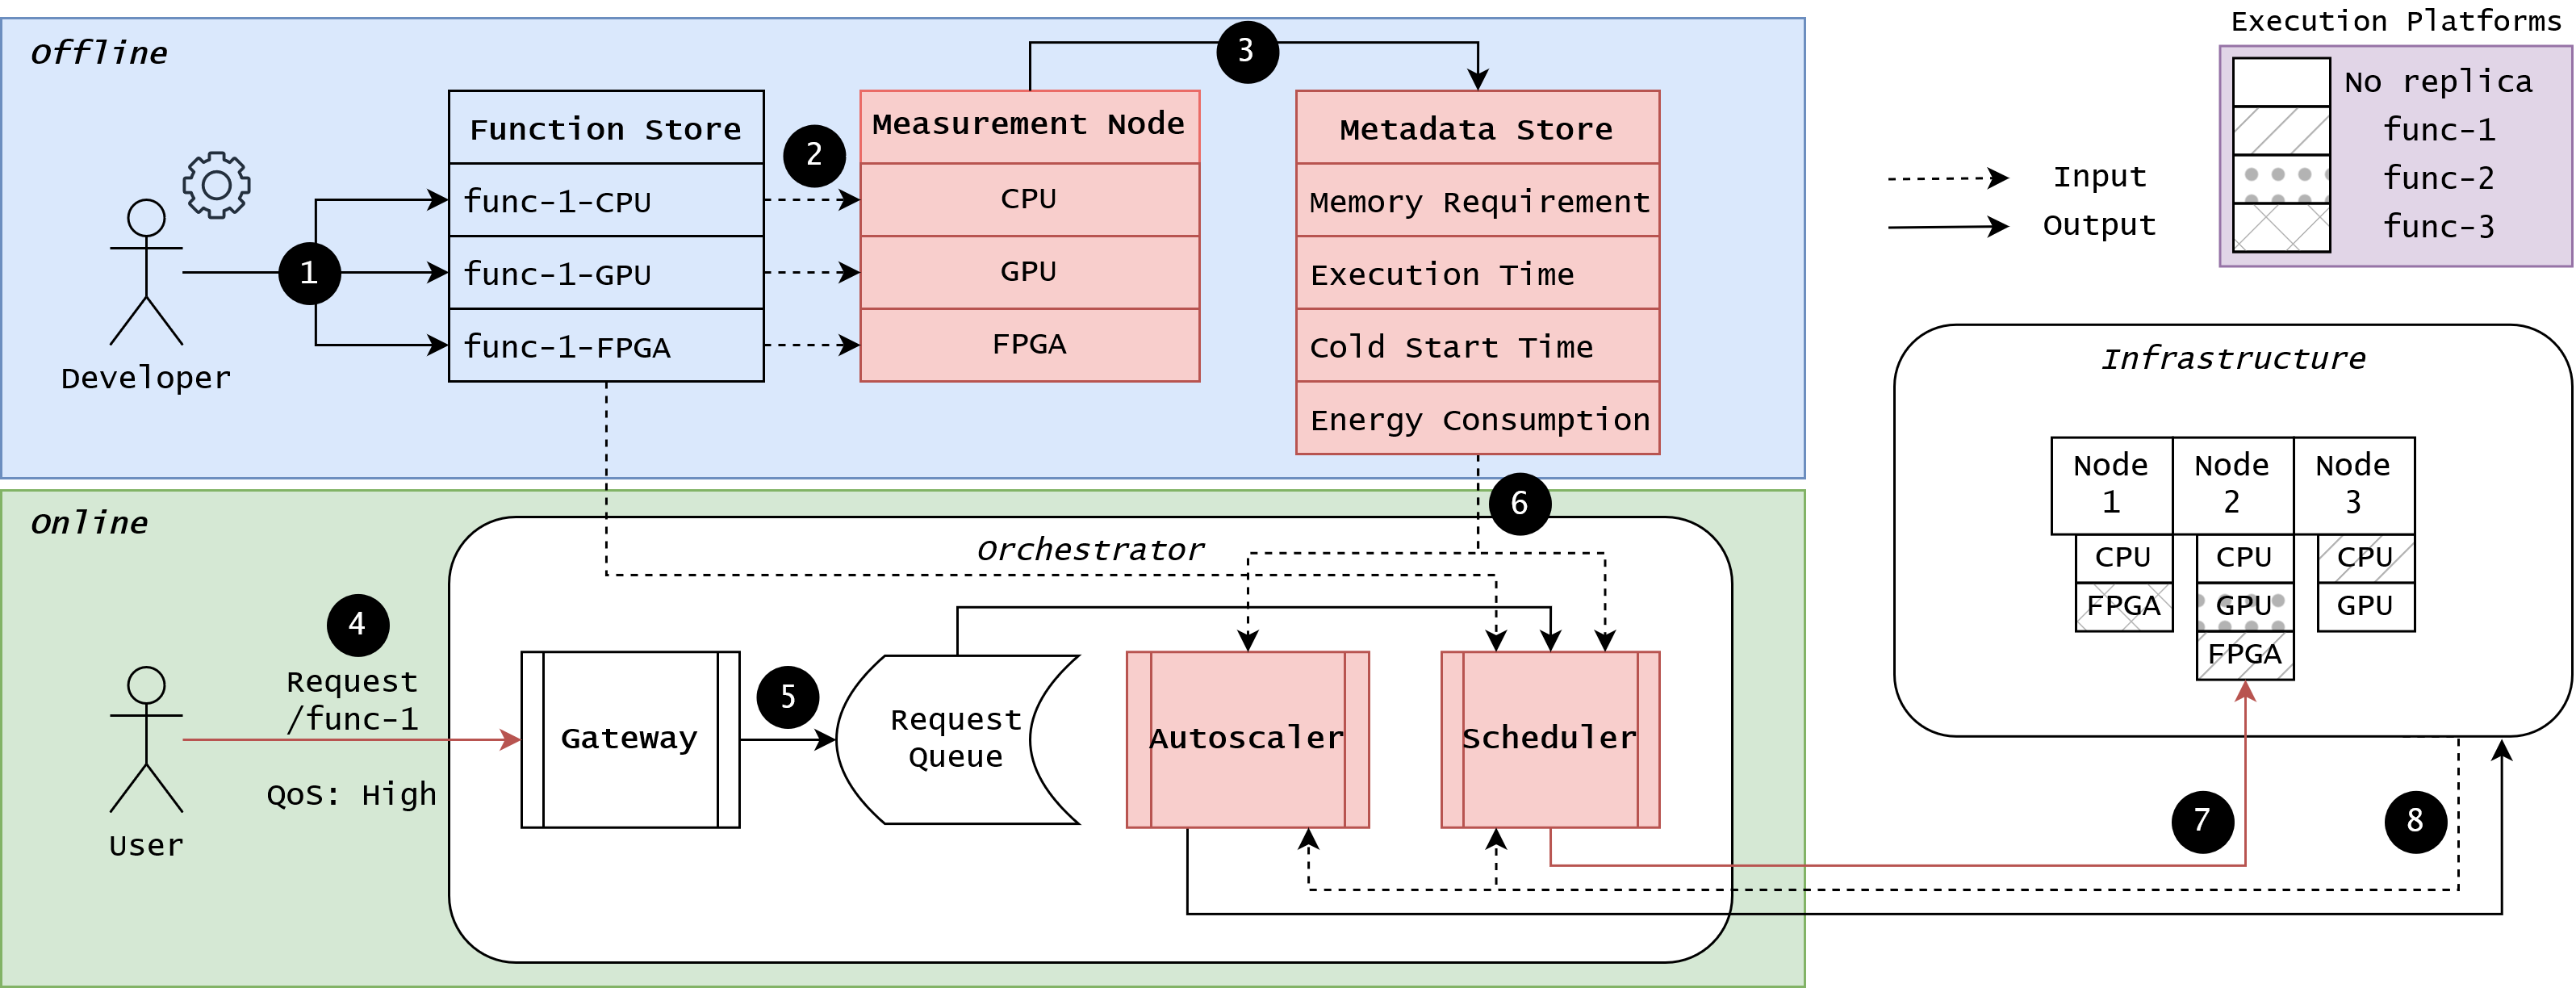
\includegraphics[width=0.8\textwidth]{5_Chapitre3/figures/placement.png}
\caption{Serverless deepfake detection platform, system overview}
\label{figure:herofake-placement}
\end{figure*}

This section introduces the used serverless platform model and the overall project. % and the lifecycle of a request. 

%Figure~\ref{figure:herofake-placement} highlights (with a red background) the two main parts of our contribution \jb{focale sur 2 point alors que le reste n'est pas encore exposé, bizarre} \vl{déplacé à la fin, mais peut-être qu'on peut juste s'en débarasser ou reformuler ?}:
%\jb{ça perturbe la lecture --> à enlever/commenter on verra après si on remet}
%\begin{enumerate}
%    \item a \textbf{measurement node}, that generates task metadata used to guide the allocation and scheduling decisions.
%    \item an \textbf{orchestrator}, that provides a gateway as an entry point for user requests, an autoscaler responsible for resources allocation, and a scheduler that places jobs on previously allocated resources;
%\end{enumerate}

\subsection{Platform model}

We consider a deepfake detection system that is deployed as a serverless application consisting of three stateless functions that achieve inference tasks on input images. These images are all RGB and $224 * 224$ pixels in size~\footnote{Note that videos are not yet considered in our project.}.

Figure~\ref{figure:herofake-placement} introduces the used platform, we differentiate between an \textit{offline} (blue blox in the figure) and an \textit{online} (green box in the figure) phase. During the offline phase, we collect metadata relative to tasks execution on the heterogeneous accelerators; during the online phase, we allocate resources and schedule tasks.

Function invocation requests from the users are received on the provider's gateway and handled by the orchestrator. In our model, a function invocation corresponds to a \textit{task}. The user selects one of the three provided models (ResNet50, VGG16 and VGG19, see Section~\ref{offline:workload}) and uses it to detect a possible deepfake on a picture.

The cloud provider's infrastructure is modeled as a set of heterogeneous \textit{nodes} (Section~\ref{model:nodes}) comprising various combinations of \textit{platforms} (Section~\ref{model:platforms}) that can execute incoming \textit{tasks} (Section~\ref{model:tasks}). 

\subsubsection{Nodes} \label{model:nodes}
A node is a server available in the service provider's infrastructure. In this work, we do not consider storage and data locality. Input data are always provided \textit{via} file upload by the user at the time of their request.
As such, the only characteristic that defines a node in our infrastructure model is the size of dedicated memory. A node consists of a set of execution platforms defined hereafter.

\subsubsection{Execution platforms} \label{model:platforms}

An execution platform is a hardware processing unit available on a node. Each platform consumes a quantity of energy in the "idle" state expressed in kilowatt-hour (kWh). When it starts executing a task, it consumes additional energy characterized by the task's properties/type: it is then in an "active" state. We differentiate "idle" and "active" time for each platform, so as to measure resources usage.
Platforms are characterized by a \textit{platform type} that encompasses the following parameters:

\begin{itemize}
    \item \textit{Hardware type} -- CPU, GPU or FPGA;
    \item \textit{Price} -- the cost of acquisition of such a platform by the cloud provider;
    \item \textit{Idle energy} -- the baseline energy consumption for the platform when it is not running any task.
\end{itemize}

\textbf{Task caching and cold start model}. We consider a simple task caching mechanism at platform-level, akin to a keep-alive mechanism~\cite{7279063}. In our system, if a platform was previously executing a task of type $t$, and a new task of the same type $t$ is scheduled on that same platform, then the cold start delay will not be incurred. However, if that same platform were to execute a task of different type $tt$, then the task will go through a cold start before entering its execution phase. Finally, if the platform was not previously allocated, the task will also experience a cold start delay.

\subsection{Overall project description}

The b{\textless\textgreater}com research institute works on a project that aims to deploy an application of deepfake detection on a private cloud. Users submit a picture to the system and when their request is fulfilled, they obtain a boolean value as a response. The application targets different classes of users -- some of them can be media or authorities with high QoS requirements, while others can be casual users tolerating a higher latency.

To differentiate between these classes of users, we propose different levels of per-request SLA. Users with higher requirements will agree to pay a higher per-request price, however if we fail to fulfill their request in the allotted response time, we will consent to a discount -- the higher the QoS level, the higher the discount. Hence, there is a strong monetary incentive for the provider to achieve QoS.

\textbf{Offline phase}. In our platform, the lifecycle of the application starts during an offline phase with the developer providing the code of their functions for different hardware architectures \Circled{1}. That code is stored in a function repository. Functions are then deployed on a measurement node \Circled{2} where they are run in order to generate metadata relative to the functions: memory requirements, execution time, cold start time and energy consumption for each function are written to a metadata store \Circled{3}. The offline phase is required to run once for a given function on a given platform, it is described in Section~\ref{offline}.

\textbf{Online phase}. When a user sends a request to the application \Circled{4}, they provide an input picture and specify their desired QoS level. The request is appended to a request queue \Circled{5} at the orchestrator level. When the scheduler pops the request from the queue, the metadata store is queried to retrieve the appropriate function metadata \Circled{6}.

The scheduler then proceeds to try to schedule a task (i.e. a function's invocation) to fulfill the request. Tasks are placed on already deployed function \textit{replicas} \Circled{7}. Such replicas can either be containers or virtual machines, i.e. sandboxed execution environments for the given function. 
Concurrently, the autoscaler monitors the request queues in all the function replicas \Circled{8}. The role of the autoscaler is to rightsize the resources allocation with regard to the fluctuations in load on each function. 
The designed scheduler and the autoscaler are described in Section~\ref{online}.

%gives further details regarding the scheduling strategy.
%Section~\ref{section:herofake-autoscaling-strategy} gives further details regarding the autoscaling strategy.
\section{Offline phase: measurement and metadata extraction}
\label{offline}
\subsection{Execution platform benchmarks}

\begin{table}[t]
\caption{Execution platform characterization}
\begin{center}
\resizebox{\columnwidth}{!}{%
\begin{tabular}{|c|c|c|c|c|}
\hline
                             \textbf{Platform} & \textbf{Hardware type}& \textbf{Price (MSRP)} & \textbf{Idle energy} \\ \hline
Intel Xeon ES-1620 v4         & CPU           & 294          & 0.067       \\ \hline
Nvidia GeForce RTX 2070 Super & GPU           & 499          & 0.010       \\ \hline
Xilinx Alveo U250             & FPGA          & 7695         & 0.030       \\ \hline
\end{tabular}%
}
\end{center}
\label{table:herofake-platforms}
\end{table}

As the usage of deep learning inference and energetic impacts grow simultaneously in computing, the power efficiency of the target devices becomes a major concern. The FPGA-based acceleration boards are described as a relevant competitor against the dominant GPU approach. Our study proposes a benchmark, using convolutional neural network (CNN)-based approaches for deepfake detection on CPU, GPU, and FPGA technologies regarding power efficiency during inference time. Our comparison includes power usage, inference speed, and accuracy using traditional CPU and GPU processing against FPGA. Those metrics are crucial for an efficient orchestration on top of heterogeneous platforms.

%For our experiments, the performance comparison has been made between a CPU, a GPU, and a FPGA. 
The used CPU was an Intel Xeon CPU ES-1620 v4 (3.5 GHz) while the GPU was an Nvidia GeForce RTX 2070 Super which can be used with the new versions of AI frameworks. Therefore, both were compatible with TensorFlow, i.e the platform used for inference. with regard to the FPGA, we used the Alveo U250, a cloud computing card from Xilinx, which is compatible with Vitis-AI~\cite{vitis-ai}. The silicon processes used for both devices are similar (12 nm for the GPU and 16 nm for the FPGA), but the GPU may get a slight advantage in this benchmark for its more advanced silicon technology.

In order to carry out the inference on the FPGA, we used Vitis-AI. At the time of this study, the latest available version (v. 2.0) has been used. Vitis-AI proposes two methods for the optimization of the models. The first one is the pruning, which consists in a reduction of the complexity of the model by a compression while removing some non-critical sections of the tree. The second one is the quantization, where we convert the 32 bits floating weights into 8 bits integer. The latter method, which is freely available, is the method we used to optimize our model before the compilation, which converts our model into DPU (Deep Learning Processing Unit) instructions.

\subsection{Workload characterization}
\label{offline:workload}

\begin{table}[t]
\caption{Workload characterization }
\centering
\resizebox{\columnwidth}{!}{%
\begin{tabular}{|c|cc|ccc|ccc|ccc|}
\hline
Task     & \multicolumn{2}{c|}{Memory (GB)} & \multicolumn{3}{c|}{Cold start (s)}                              & \multicolumn{3}{c|}{Execution time (s)}                         & \multicolumn{3}{c|}{Energy (mWh)}                            \\ \hline
         & \multicolumn{1}{c|}{CPU}  & GPU  & \multicolumn{1}{c|}{CPU}   & \multicolumn{1}{c|}{GPU}   & FPGA   & \multicolumn{1}{c|}{CPU}   & \multicolumn{1}{c|}{GPU}   & FPGA  & \multicolumn{1}{c|}{CPU}  & \multicolumn{1}{c|}{GPU}  & FPGA \\ \hline
ResNet50 & \multicolumn{1}{c|}{1.3}  & 3.3  & \multicolumn{1}{c|}{1.232} & \multicolumn{1}{c|}{2.340} & 9.952  & \multicolumn{1}{c|}{0.124} & \multicolumn{1}{c|}{0.024} & 0.009 & \multicolumn{1}{c|}{3.11} & \multicolumn{1}{c|}{1.7}  & 0.5  \\ \hline
VGG16    & \multicolumn{1}{c|}{1.8}  & 3.3  & \multicolumn{1}{c|}{2.514} & \multicolumn{1}{c|}{4.641} & 14.528 & \multicolumn{1}{c|}{0.143} & \multicolumn{1}{c|}{0.046} & 0.010 & \multicolumn{1}{c|}{4.34} & \multicolumn{1}{c|}{3.43} & 0.55 \\ \hline
VGG19    & \multicolumn{1}{c|}{1.9}  & 3.4  & \multicolumn{1}{c|}{2.559} & \multicolumn{1}{c|}{4.641} & 14.758 & \multicolumn{1}{c|}{0.167} & \multicolumn{1}{c|}{0.048} & 0.012 & \multicolumn{1}{c|}{5.16} & \multicolumn{1}{c|}{3.58} & 0.65 \\ \hline
\end{tabular}
}%
\label{table:herofake-tasks}
\end{table}

For the purpose of this study, three popular models have been trained. The first one is based on residual networks (ResNet50), which uses residual blocks and can be efficiently trained~\cite{NEURIPS2019_7716d0fc}. The second one is VGG16 (VGG for Visual Geometry Group), which uses only convolutions as blocks~\cite{DBLP:journals/corr/SimonyanZ14a} and the third one is VGG19, a variant of VGG16 with three additional layers~\cite{biom10070984}. Those networks are trained on a GPU, as training is not the subject of this study.

\subsection{Performance measurements}

\begin{figure}[t]
\centering
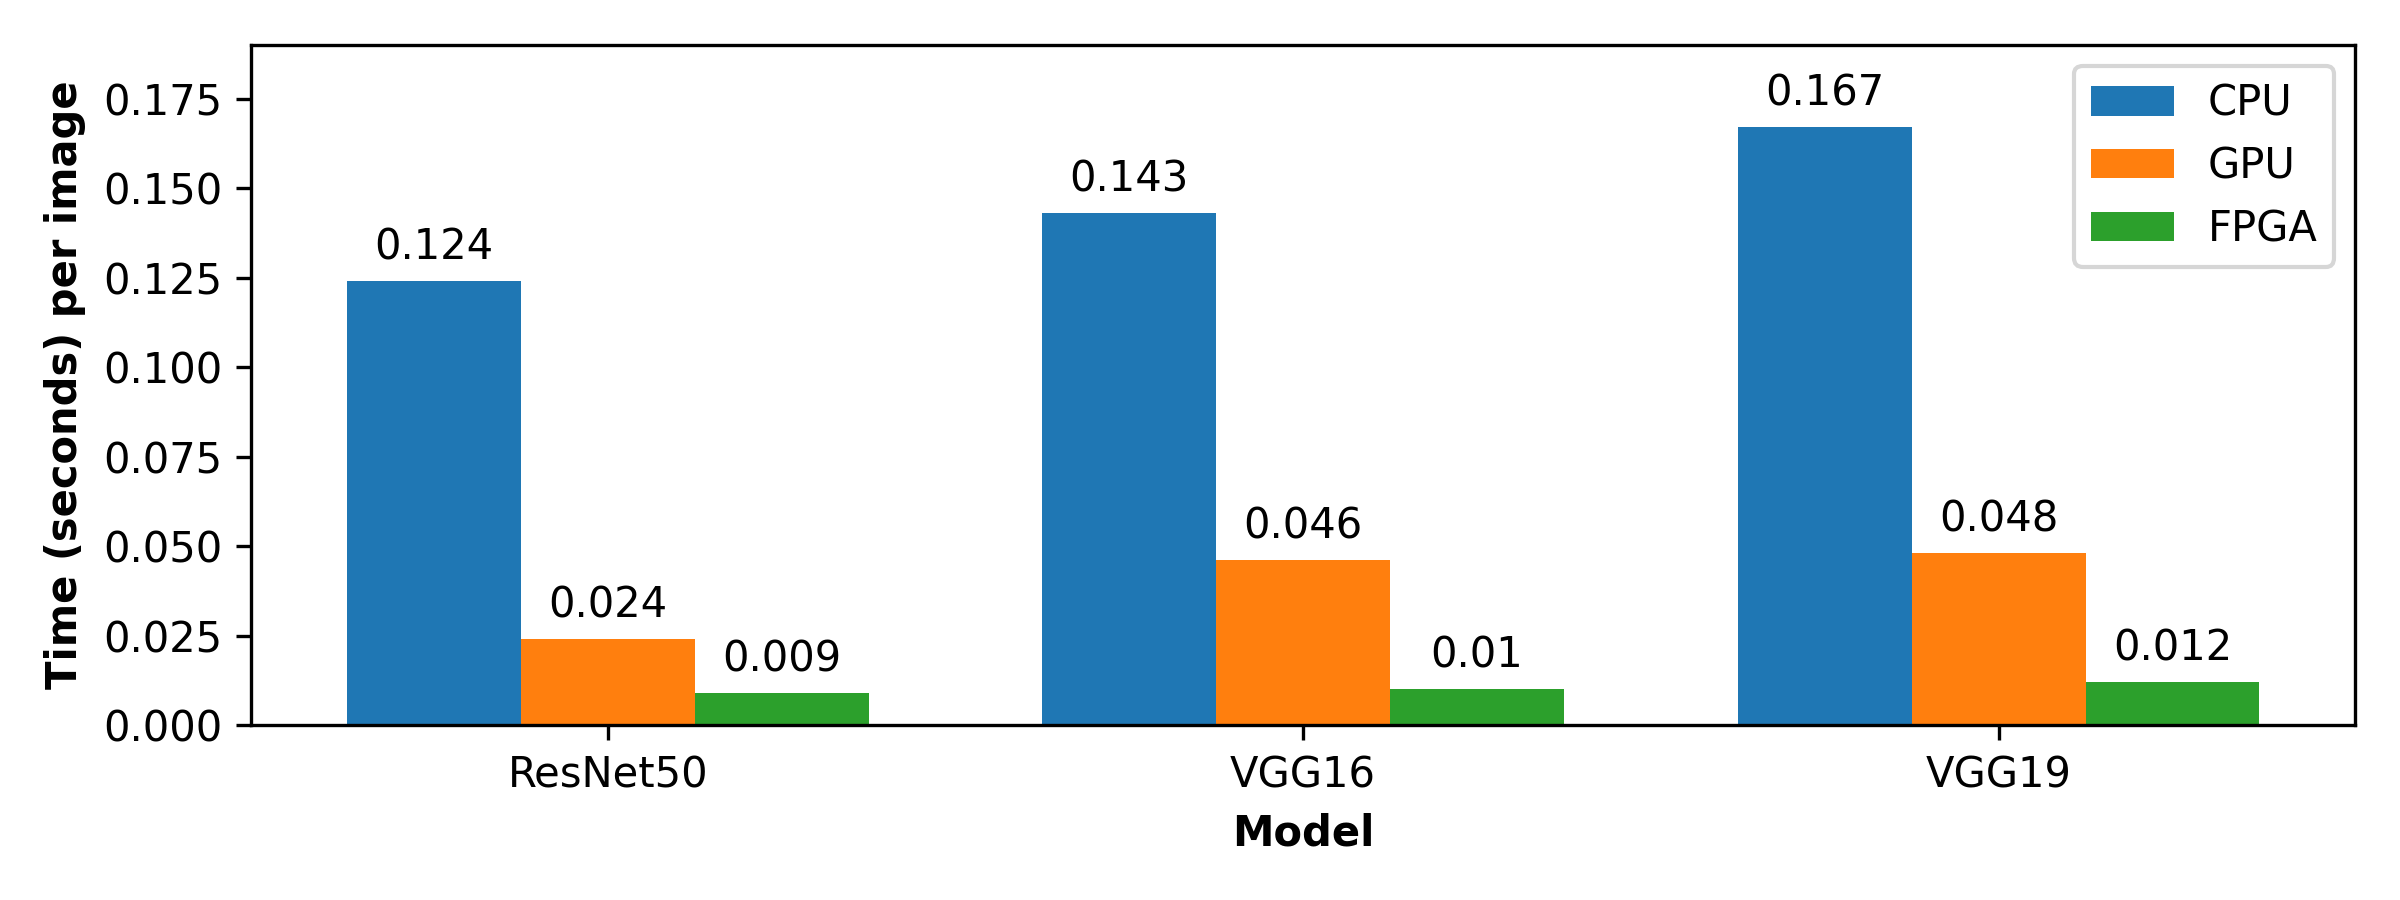
\includegraphics[width=\columnwidth]{5_Chapitre3/figures/characterization/time_of_inference_1_image.png}
\caption{Inference time for one image with ResNet50, VGG16 and VGG19.}
\label{figure:herofake-time-inference}
\end{figure}

%The first consideration in this benchmark is to compare the performance in terms of inference time with the different technologies. 
As the FPGA acceleration card is intended to be more efficient than a CPU or a GPU~\cite{5272532}, making a comparison of the inference time with these three technologies is a first requirement to enable the comparison of the energy cost per image. The performance evaluation in terms of execution time was realized with the same 10,000 images for the three different models. We built a two classes deepfake dataset, the real ones from the CelebA dataset~\cite{https://doi.org/10.48550/arxiv.1411.7766}, and the fake ones generated using a Generative Adversarial Network (GAN)~\cite{jimaging7080128}. The quantization and compilation of the graph was performed with Vitis-AI in order to run it on the FPGA. Only considering the inference time, it turned out that on the three tested models (ResNet50, VGG16 and VGG19), the FPGA is 13.08 to 13.79 times faster than the CPU but also 2.52 to 4.48 times faster than the GPU (see Figure~\ref{figure:herofake-time-inference}).

\subsection{Energy consumption measurements}

\begin{figure}[t]
\centering
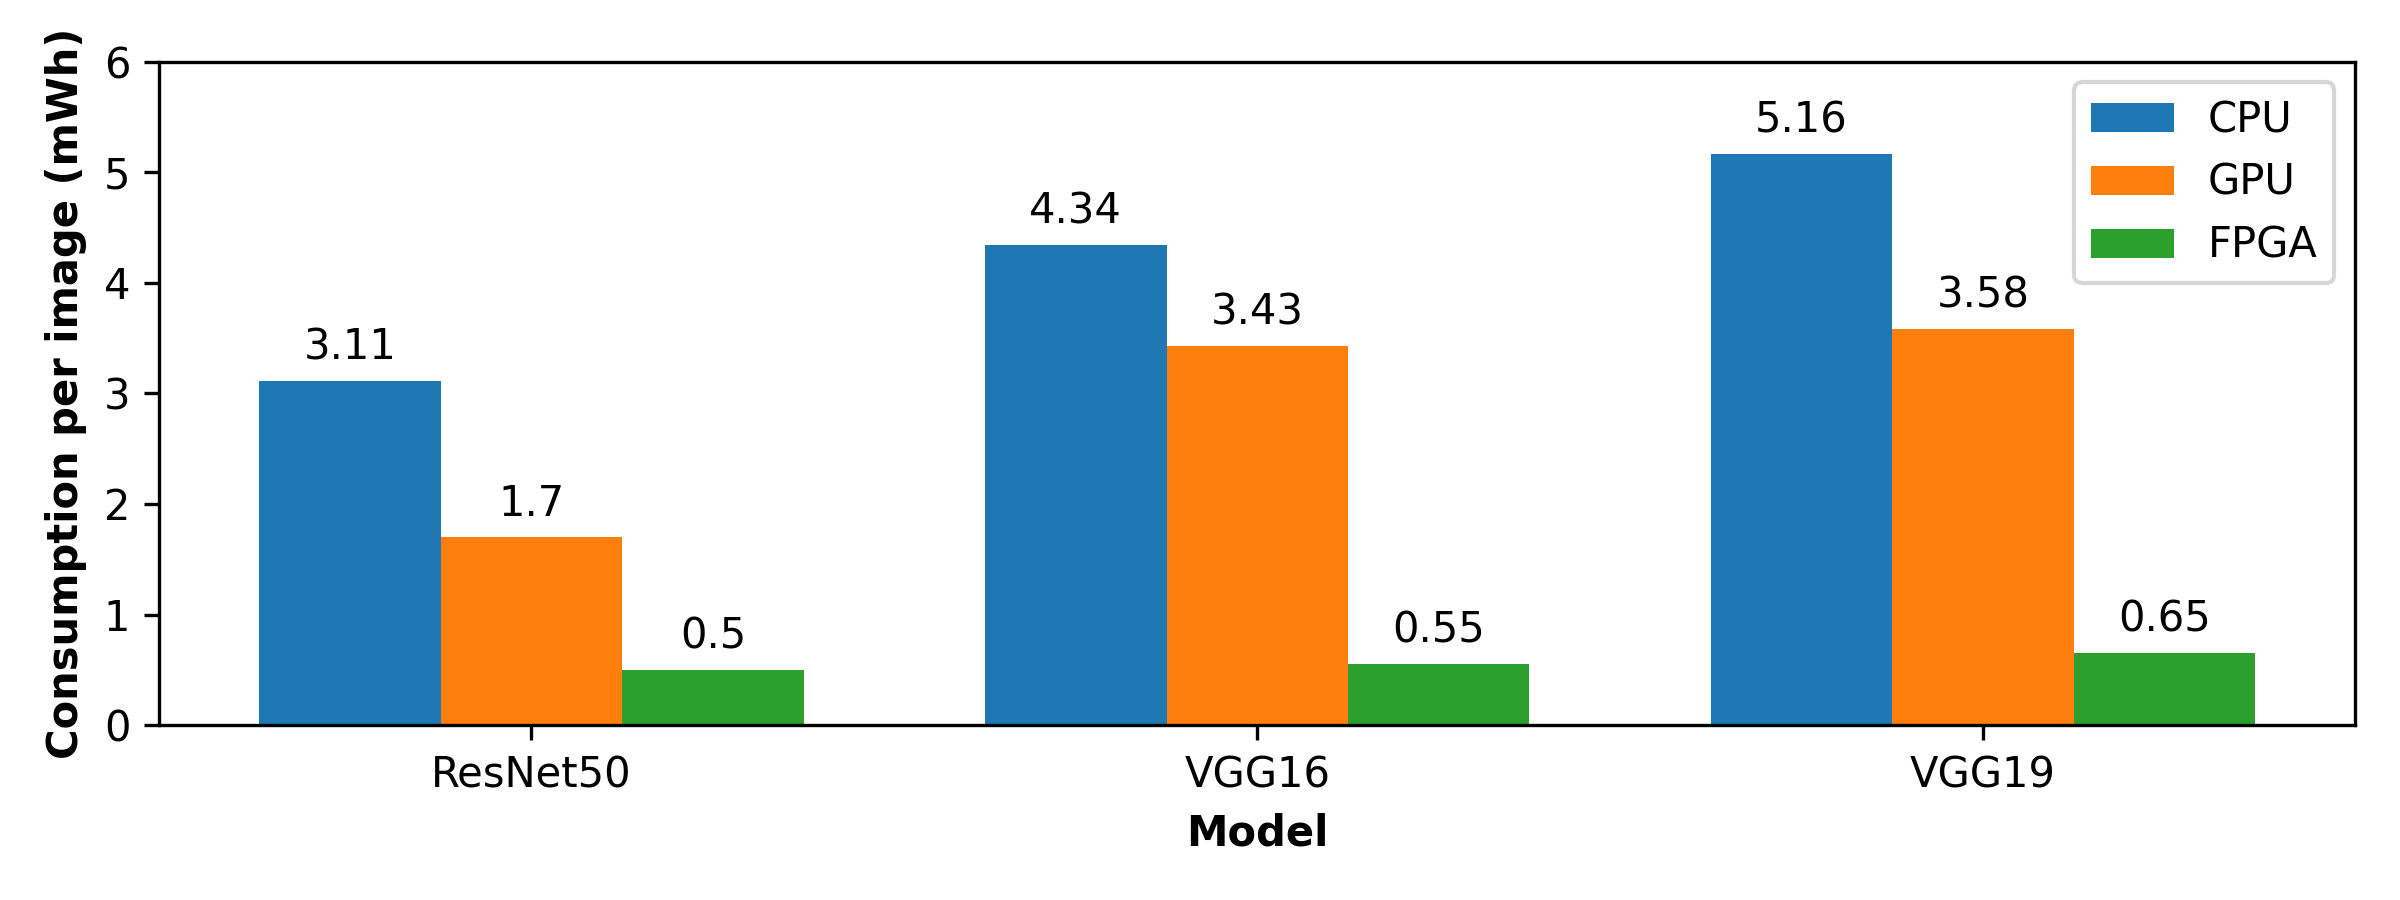
\includegraphics[width=\columnwidth]{5_Chapitre3/figures/characterization/consumption_per_image.png}
\caption{Energy consumption of inference per image (mWh).}
\label{figure:herofake-consumption-per-image}
\end{figure}

The instant power consumption measured during inference is  the overall consumption of the machine (including CPU, memory, mainboard, and power supply) while performing the inference. 
Measurements have been done using a power distribution unit (PDU) (Raritan PX3-5190R) which is able to monitor instant power and energy consumption of the server (Dell Precision T5810). The results show that inference on CPU yields the lowest instant power consumption. This result is quite expected as the inference on GPU or FPGA also includes power consumption from the CPU. % the power usage of the GPU and the FPGA adds-up to the CPU power.


However, the sole instant power consumption does not reflect the total cost advantage of each platform properly. The execution time needed to process all the images must be considered. The relevant measurement is energy cost per image. The energy consumption has been measured in kilowatt-hour (kWh) for the 10,000 images, then converted into milliwatt-hour (mWh) per image. From that point of view, it is clear that the FPGA is the most energy efficient with regard to the execution time, consuming 6.2 to 6.9 times less than the CPU and 3.3 times to 6.2 times less than the GPU (see Figure~\ref{figure:herofake-consumption-per-image}).

\subsection{Discussion}

\begin{figure}[t]
\centering
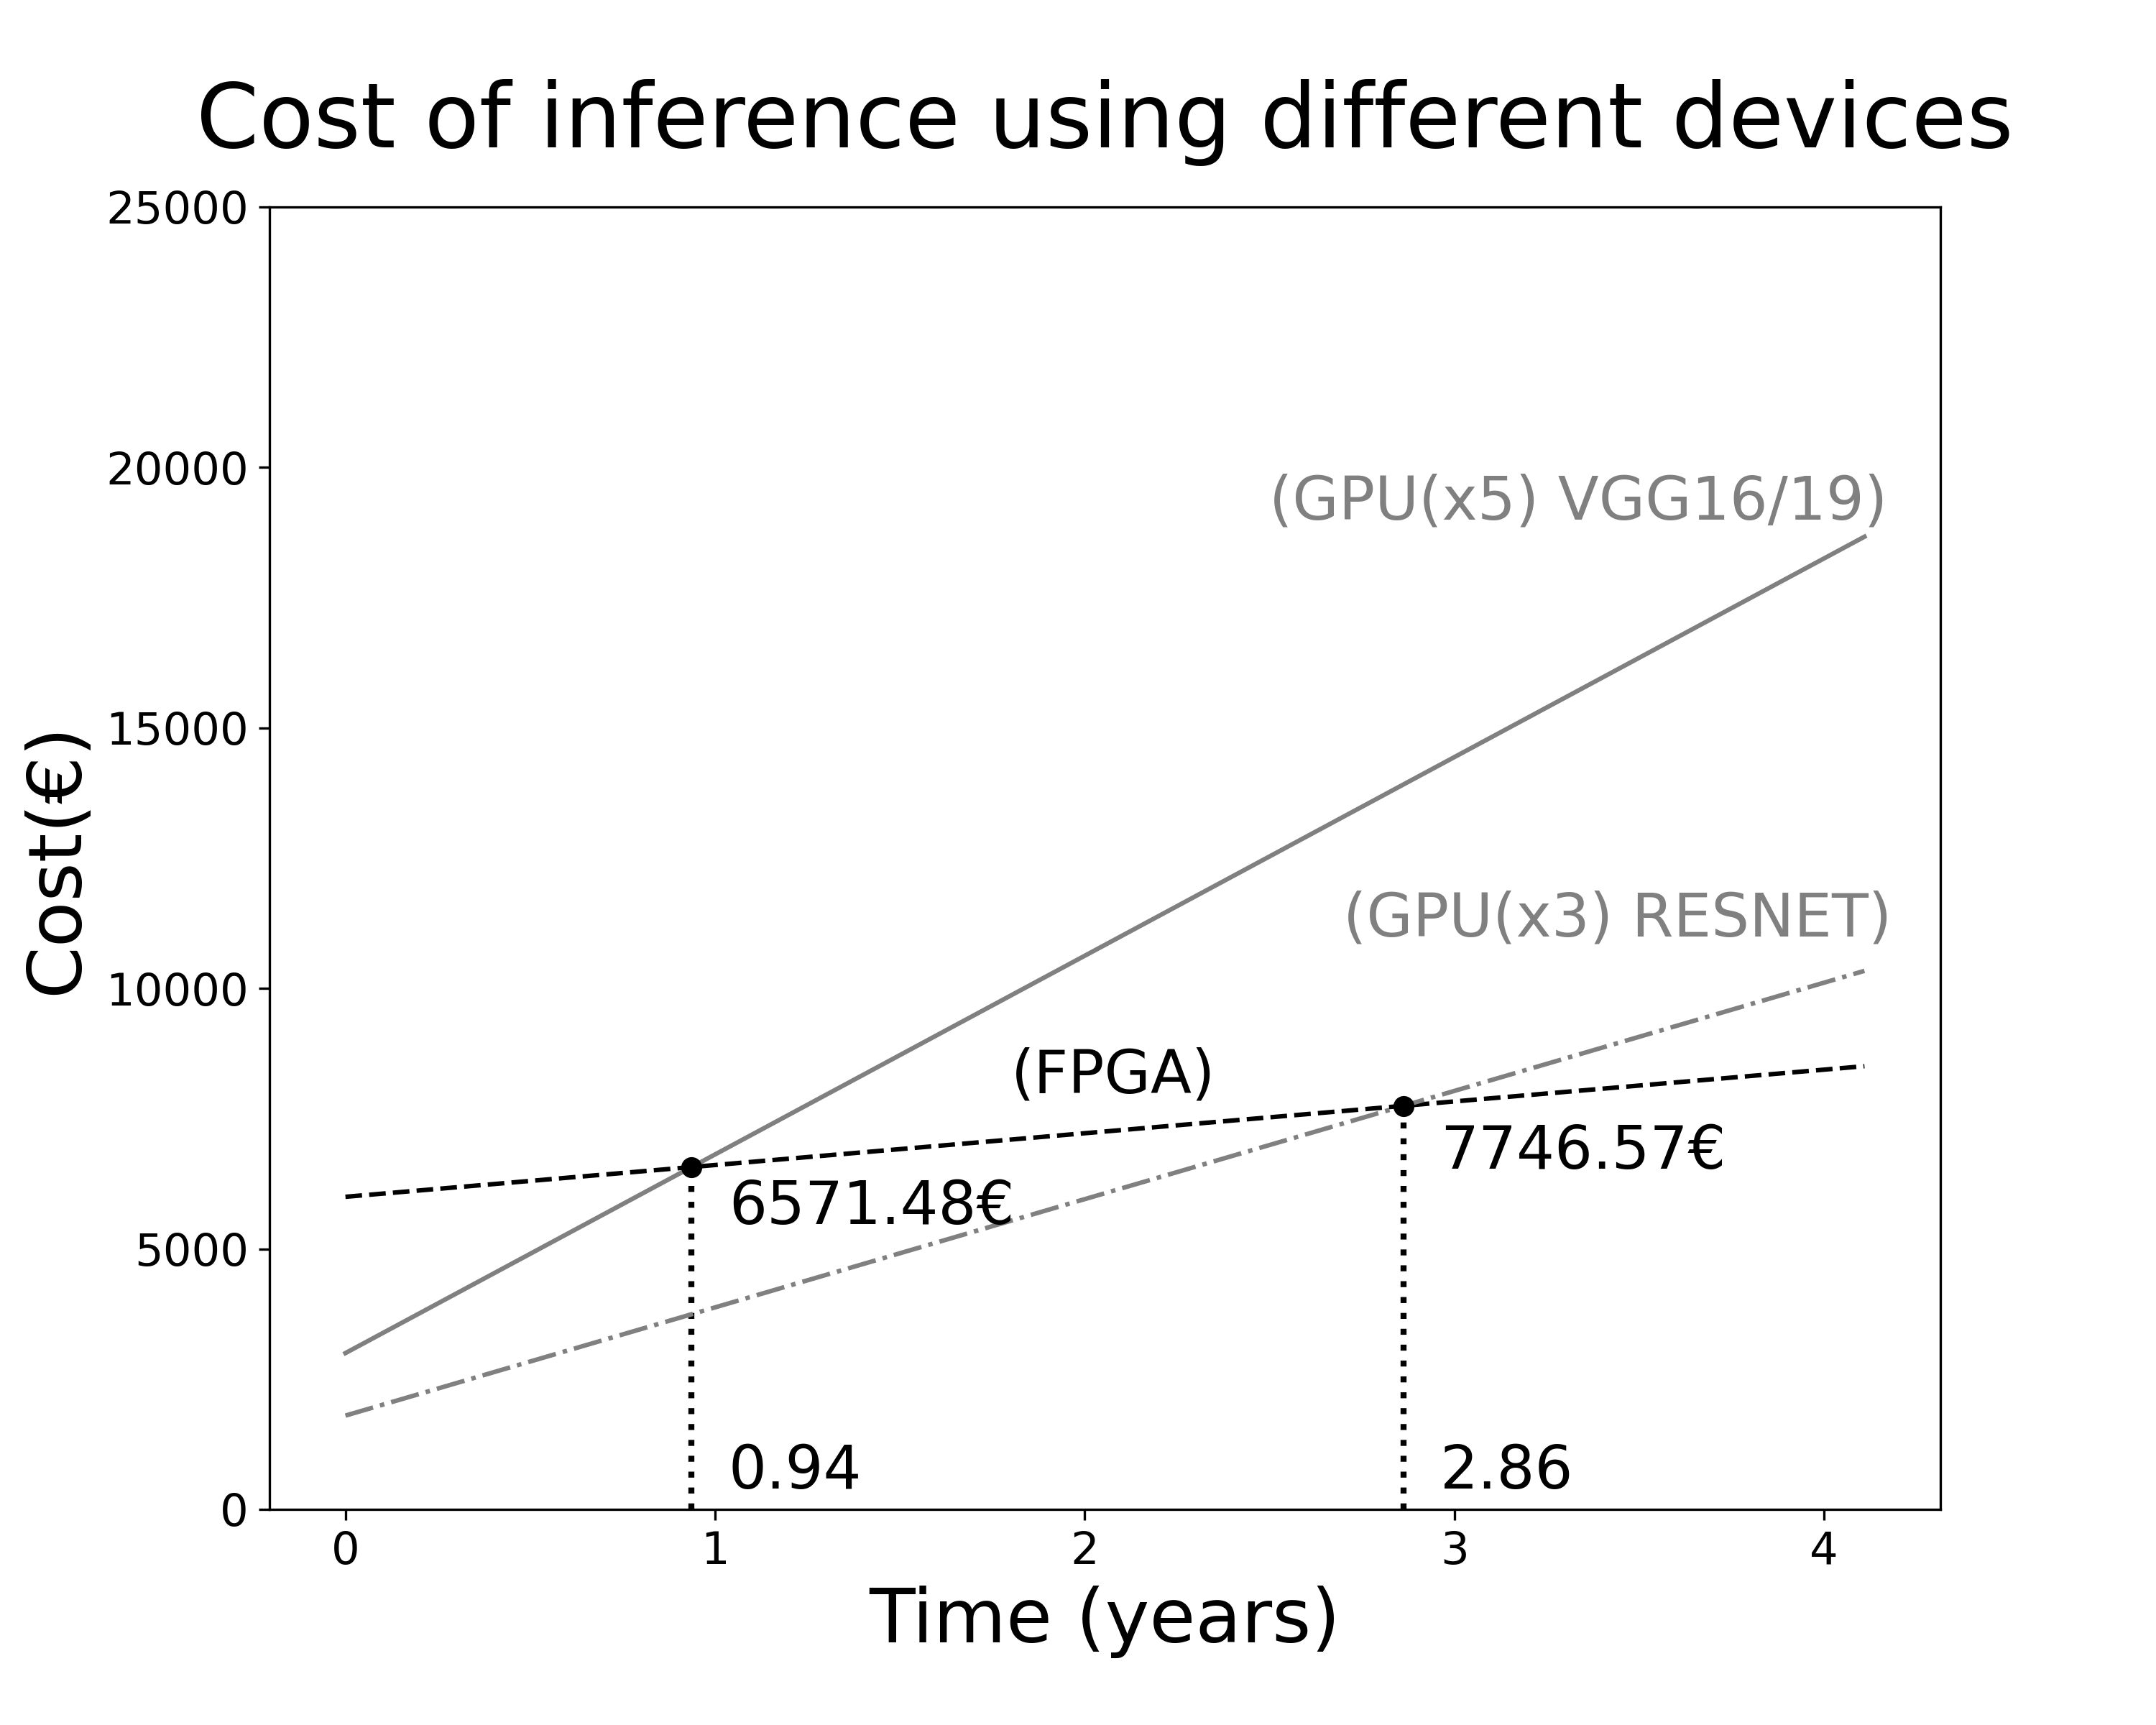
\includegraphics[scale=0.2]{5_Chapitre3/figures/characterization/cost_devices_time.png}
\caption{Total cost of inference on selected devices over time.}
\label{figure:herofake-cost-over-time}
\end{figure}

The results of this benchmark show a clear advantage of the inference on FPGA regarding performance and energy efficiency. The gains in performance are significant, especially with deep learning networks with higher complexity~\cite{8782524}. Computing resources based on servers equipped with FPGA acceleration boards, instead of GPU acceleration boards, would benefit from these advantages.

The raw energy consumption of the inference device does not reflect the total cost of the solution. Indeed, one must also include the cost of the equipment itself. This is a major point in the comparison between GPU and FPGA, because there is a price gap between the two technologies: the GPU (RTX 2070 Super) being used for this benchmark was introduced around 600€, while the FPGA (Alveo U250) is sold around 6000€. The cost of the electric energy to perform the inference is very low (we used the European average of 0.1833€ per kWh as proposed in~\cite{energy-price}), compared to the initial cost of the device: the runtime needed to benefit from the cost advantage of the FPGA is in the order of several months of continuous operation. Figure~\ref{figure:herofake-cost-over-time} depicts cumulative cost (in euros) of the usage of a server with either GPU or FPGA acceleration versus time (in years). Our cost estimate includes the number of GPU needed with their cost to equalize the FPGA performances and uses a 2x factor~\cite{shehabiUnitedStatesData2016}, to account for the total power consumption of the infrastructure (mainly cooling and networking). The FPGA can become a cost effective solution after a few months for complex CNNs. For networks with lower complexity, the cost advantage of the FPGA is reached after more than two years.

\begin{figure}[t]
\centering
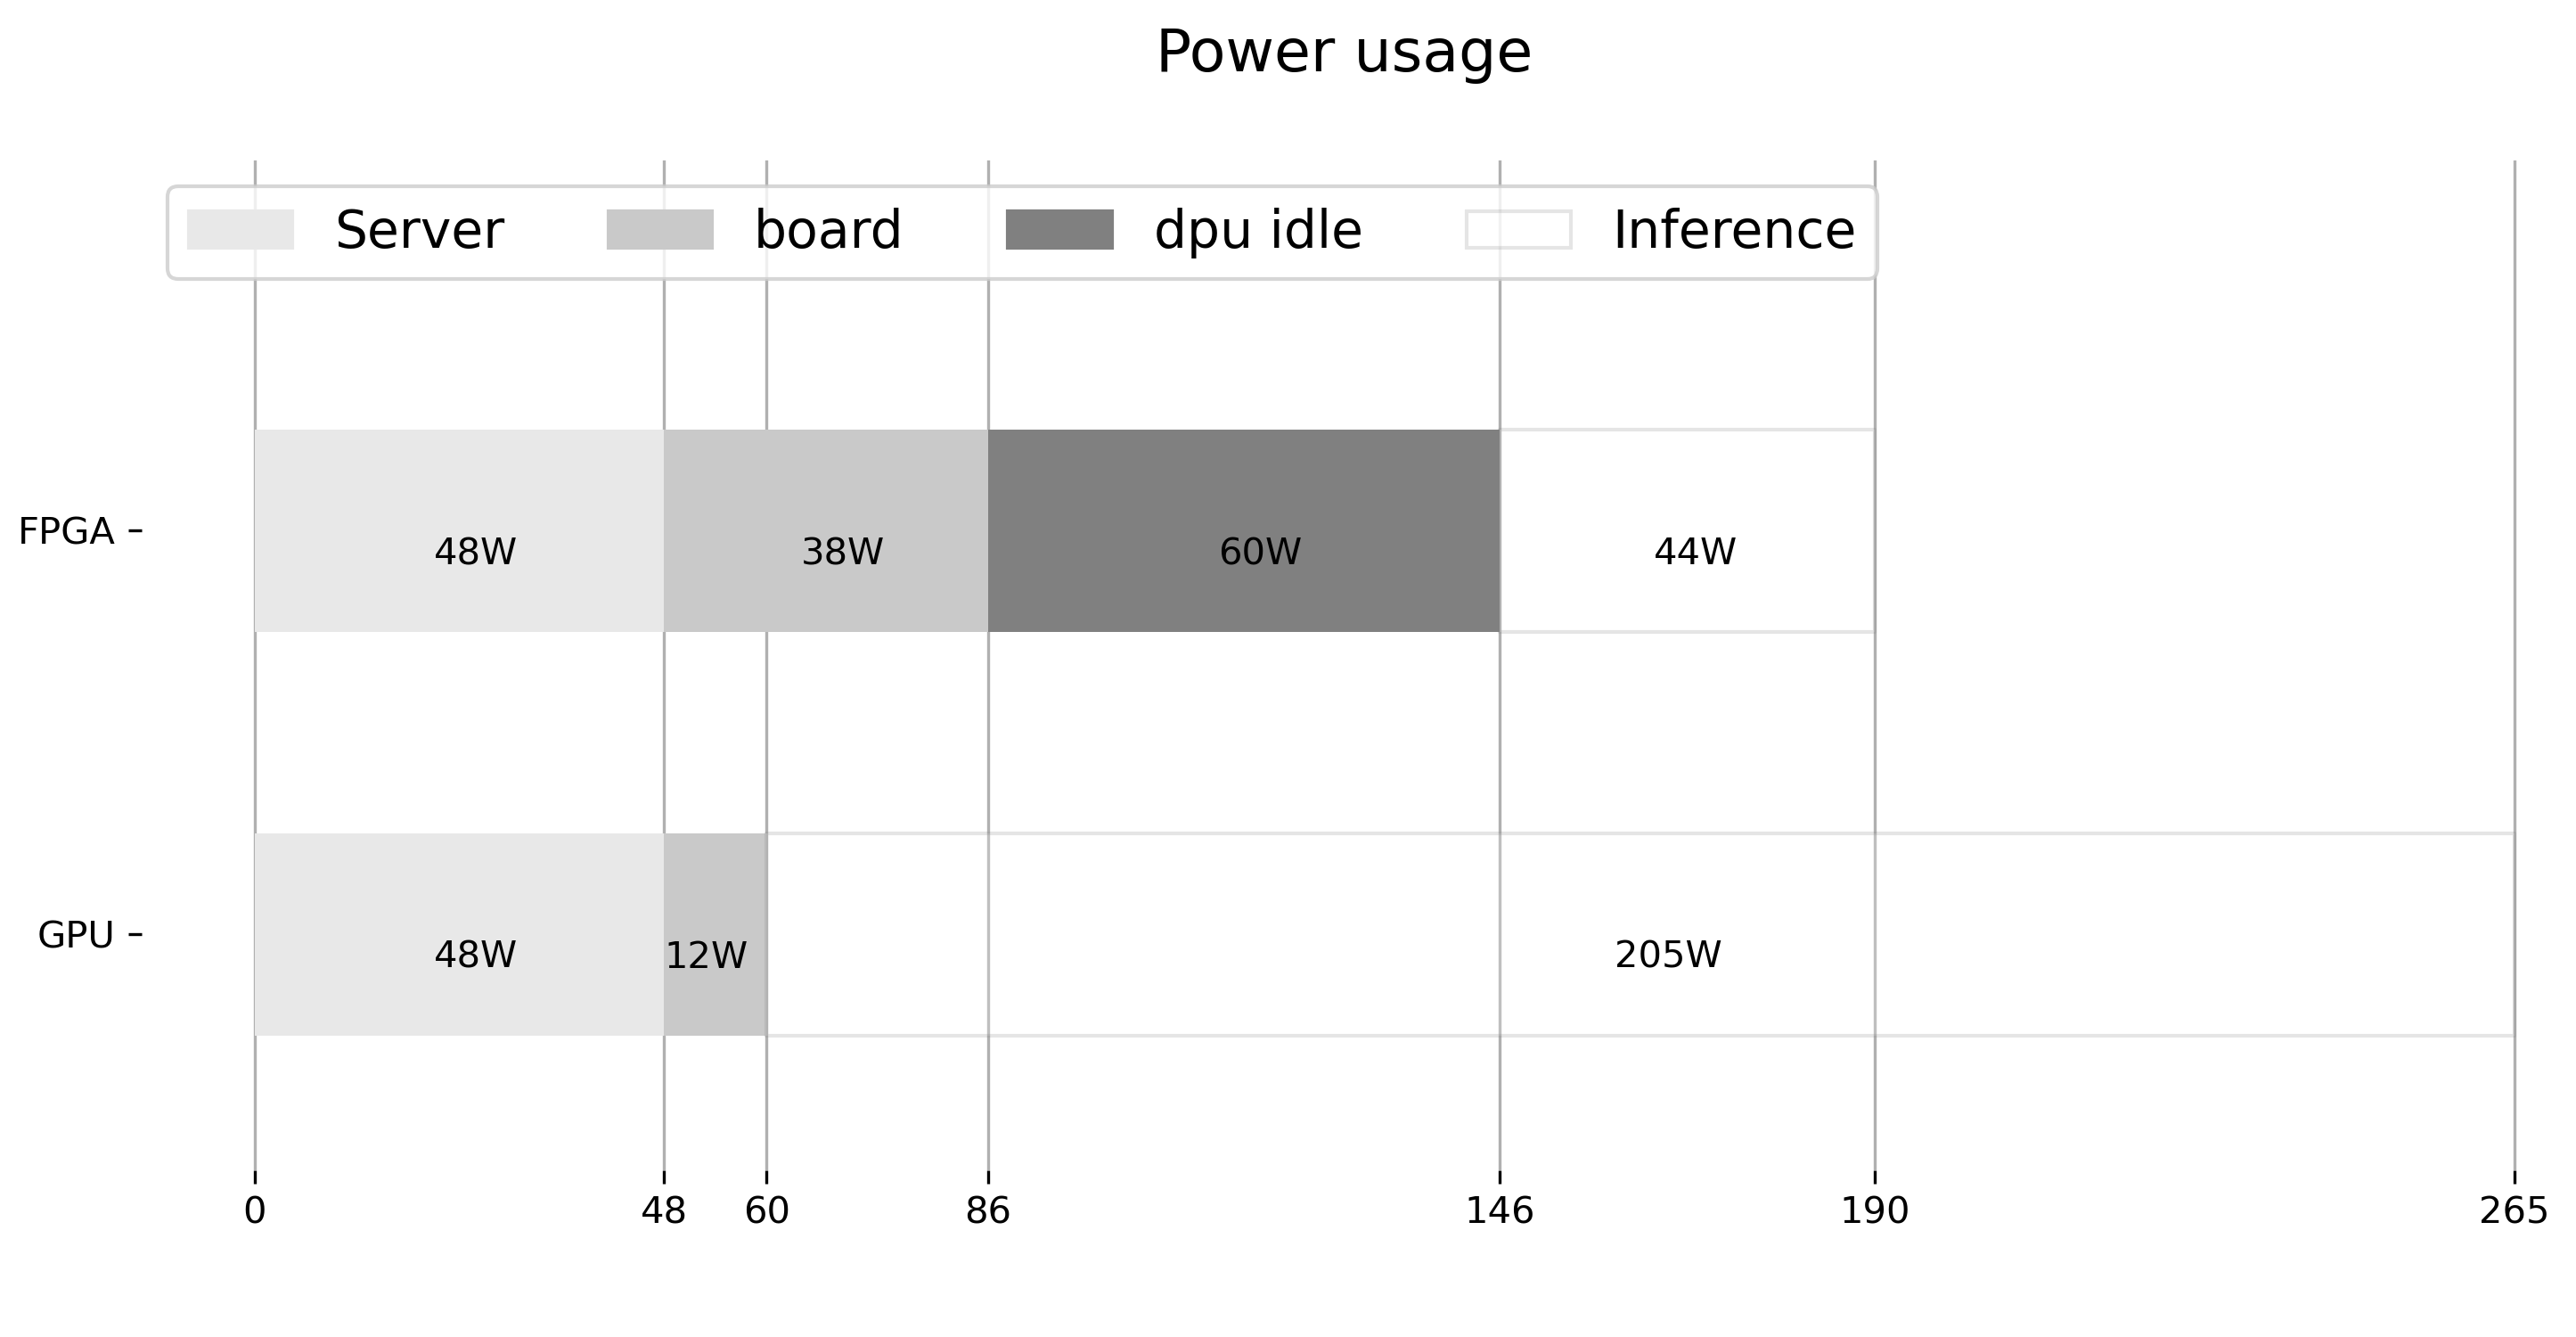
\includegraphics[width=\columnwidth]{5_Chapitre3/figures/characterization/power_usage.png}
\caption{Power usage breakdown for FPGA and GPU.}
\label{figure:herofake-power-usage}
\end{figure}

The previous analysis is valid in the situation where the inference is always performed at full load. Indeed when breaking down the power consumption of the GPU between idle power and inference power, it is clear that the GPU is able to dynamically scale its power usage with the intensity of the processing. The FPGA on the other side seems to have very limited power management. Once the DPU design is loaded into the device, its power usage at idle remains very high (see Figure. \ref{figure:herofake-power-usage}). Adding to the 38W of the FPGA board power, there is indeed a residual 60W power consumption when the DPU is idle. Even though further evolution of the DPU implementation on the FPGA may fix this issue (like reducing clock tree activity when idle), this has an impact on the total cost and must be considered if the device is not always used at full load. With only 12W of idle power, the GPU is a better candidate when full-load device usage cannot be guaranteed.

As the trend towards CNNs with more complexity continues~\cite{8807741}, using the most efficient devices will become a major challenge. The FPGA solution offers a new option to perform inference. However, FPGAs are not a drop-in replacement for GPUs yet: the compilation flow remains complex and time-consuming. A trade-off between the flexibility of the GPUs and the efficiency of the FPGAs will have to be made. The next section discusses a first orchestrator that considers the above-mentionned characterization for allocating and scheduling heterogeneous resources.

\section{Online phase: Autoscaling and scheduling}
\label{online}
In this section, we formulate the problem that our contribution addresses, and give a detailed description of our model. Finally, we present a formal description of our strategy for the autoscaling of resources and scheduling of tasks. 

%In order to optimize the placement of tasks following incoming requests, we propose an online scheduler that takes into account the level of QoS requirements associated with each task. To meet these requirements, the autoscaler has to be able to opportunistically allocate hardware accelerators according to the task's deadline, given its characteristics on each execution platform. These characteristics are made available in the task's metadata.

\subsection{Serverless resource orchestration challenges}

Scheduling workloads in the serverless paradigm is a two-fold problem: providers have to dynamically handle resource allocation (i.e. managing resources pools when scaling the number of replicas for an application) and job placement (i.e. mapping tasks to existing replicas).

Increasing the replica count introduces a performance challenge: when a new replica is spun up, be it as a container or a virtual machine, the execution sandbox has to go through its initialization phase. This is called a "cold start".

Commercial solutions such as AWS Lambda often avoid the cold start problem by maintaining pools of pre-warmed sandboxes~\cite{vahidiniaColdStartServerless2020}. These virtual machines (VMs) or containers are started in anticipation and paused in a post-initialization state. When activity resumes, incoming requests can be served without suffering a cold start delay, at the expense of resources multiplexing on the provider side. While this solution allows reducing, or even eliminating cold start delays, it takes a toll on the provider's resources multiplexing capacity~\cite{hellersteinServerlessComputingOne2019} and raises the total cost of ownership (TCO).

% Load is unpredicTable~\cite{shahradServerlessWildCharacterizing}
%\begin{itemize}
%    \item stochastic barrier;
%    \item need for an online solution.
%\end{itemize}

%Furthermore, Machine Learning as a Service (MLaaS) applications exhibit highly fluctuating load~\cite{gujaratiSwayamDistributedAutoscaling2017}, thus reinforcing the argument that overprovisioning resources for such a service is not a viable solution.

Furthermore, Machine Learning as a Service (MLaaS) applications exhibit highly fluctuating load~\cite{gujaratiSwayamDistributedAutoscaling2017}, thus reinforcing the argument that a reactive resource allocation strategy is necessary to rightsize the infrastructure. However, as the execution time of inference tasks is in the ballpark of hundredths to tenths of a second, while the initialization time of sandboxes can range between hundredths of a second to seconds~\cite{mancoMyVMLighter2017}, we need a mechanism to avoid incurring huge latency costs to the execution of functions.

% Service level is not guaranteed
%\begin{itemize}
%    \item resources availability over time is not the most relevant QoS metric;
%    \item risks of overcommitting resources.
%\end{itemize}

Mission critical tasks require service level guarantees from the provider. SLAs in cloud computing typically consist in agreeing on a resource availability rate over time; if the provider fails to meet this agreement, a discount is offered to the customer. While this may work for reserved resources, we can see that it does not make sense in the serverless paradigm. The ability to guarantee task response time would allow a serverless provider to achieve per-invocation SLAs~\cite{zhangMArkExploitingCloud}.

% Cloud resources are heterogeneous
%\begin{itemize}
%    \item various levels of performance;
%    \item various levels of cost.
%\end{itemize}

A possibility to improve performance-cost ratios is to make use of hardware accelerators. Despite being a costly investment (see Figure~\ref{figure:herofake-cost-over-time}), these devices can achieve important speedups for parallel tasks (see Figure~\ref{figure:herofake-time-inference}), thus improving function response time, with a decreased cost in energy (see Figure~\ref{figure:herofake-consumption-per-image}).

\subsection{Task model} \label{model:tasks}

\begin{table}[t]
    \caption{Notation dictionary}
    \begin{center}
    \begin{tabular}{|c|L|}
    \hline
    \textbf{Notation} & \textbf{Description} \\ \hline
    $f_{N, P}$ & A function $f$ scheduled to run on a platform $P$ available on node $N$ \\ \hline
    $QP$ & QoS penalty \\ \hline
    $QD$ & QoS deviation \\ \hline
    $WET$ & Worst execution time \\ \hline
    $TT$ & Task total time \\ \hline
    $WT$ & Wait time \\ \hline
    $CST$ & Cold start time \\ \hline
    $ET$ & Execution time \\ \hline
    $EC$ & Energy consumption \\ \hline
    $HP$ & Hardware price \\ \hline
    $TC$ & Task consolidation \\ \hline
    $Q$ & Task queue on a replica \\ \hline
    $replicaCount_{f}$ & Size of the replica pool in the system for a function $f$ \\ \hline
    $concurrency_{f}$ & Average number of in-flight requests for a function $f$ \\ \hline
    $threshold$ & Concurrency threshold for function replicas in vanilla Knative \\ \hline
    $replicaCount_{f, h}$ & Size of the replica pool for a function $f$ on hardware type $h$ \\ \hline
    $concurrency_{f, h}$ & Average number of in-flight requests for a function $f$ on replicas of hardware type $h$ \\ \hline
    $x_{f, h}$ & Concurrency threshold for a function $f$ on a replica of hardware type $h$ \\ \hline
    $scaleCost_{{f}_{N, P}}$ & Cost of creating a new replica for function $f$ on a platform $P$ available on node $N$ \\ \hline
    $schedCost_{{f}_{N, P}}$ & Cost of scheduling an execution of function $f$ on a platform $P$ available on node $N$ \\ \hline
    \end{tabular}
    \label{table:herofake-notation}
    \end{center}
\end{table}

Applications are composed of functions. A function execution is called a \textit{task}. In this work, there are no dependencies between these tasks: the application is made up of pure, stateless functions. The events that trigger the execution of a task arrive in the system at a random, bounded interval. We formulate the hypothesis that a request always succeeds and leads to the execution of a \textit{task} (an instance of a \textit{function}). When a task has started its execution on its allocated platform, it runs for the totality of its execution time. We do not consider preemption or failures in this contribution: a task always finishes its execution successfully, albeit its response time can exceed its QoS requirements. We do not consider possible interference between workloads on the same node~\cite{dartoisInvestigatingMachineLearning2021}. 

We consider tasks that can indiscriminately be executed on heterogeneous execution platforms. In the context of our specific case study, implementation of the different functions has been done by hand for each platform; however, work exists to allow automatic cross-compilation to heterogeneous architectures~\cite{hortaXartrekRuntimeExecution2021, 10.1145/3445814.3446699}. The following metadata have been measured for each function, on each execution platform: 

%In our task model, a \textit{vector} \jb{pas clair cettte histoire de vecteur}expresses a value that can be different according to the execution platform (CPU, GPU or FPGA) allocated for the task's execution. Each function is associated with its metadata:

\begin{itemize}
    \item \textit{Memory requirements} -- the quantity of memory (in GB) allocated for the task;
    \item \textit{Cold start duration} -- the duration of sandbox initialization when running the task on a platform that does not have the function in cache;
    \item \textit{Execution time} -- the expected duration of effective execution of the task, excluding its initialization phase;
    \item \textit{Energy consumption} -- the difference between idle and active energy incurred by the execution platform when it runs the task.
\end{itemize}

Equation~\ref{eq:herofake-HRO-total-time} breaks down the expected response time for the execution of a function $f$ on a platform $P$ on node $N$.
\begin{equation}
\begin{split}
%\resizebox{0.80\columnwidth}{!}{%
    %\begin{math}
    {TT}_{{f}_{N, P}} = {WT}_{{f}_{N, P}} + {CST}_{{f}_{N, P}} + {ET}_{{f}_{N, P}}
    %\end{math}%
%}
\end{split}
\label{eq:herofake-HRO-total-time}
\end{equation}

Where:
\begin{itemize}
    \item ${WT}_{{f}_{N, P}}$ is the duration of the scheduling decision, including the time spent by the user request in the queue;
    \item ${CST}_{{f}_{N, P}}$ is the duration of initialization for the function invocation, including its potential cold start time; 
    \item ${ET}_{{f}_{N, P}}$ is the execution time of the function on the platform.
\end{itemize}

We propose different levels of QoS depending on users' needs in terms of guarantees on execution time. Each level of QoS presents a different \textit{duration deviation} (noted $QD$ in Equation. ~\ref{eq:herofake-task-penalty}) -- a factor by which the worst execution time for a function is multiplied to give an upper bound on the execution time of this function for this QoS level.

Predicted function execution time is always based on the worst execution time (noted $WET_{f}$), e.g. a task's execution time when scheduled on the execution platform showing the least level of performance for said function:

\begin{equation}
\begin{split}
    \forall \, (N, P), \, WET_{f} = \max ET_{N, P}
\end{split}
\label{eq:herofake-task-wet}
\end{equation}

After a task is scheduled on an execution platform, it will go through its total time of execution described in equation \ref{eq:herofake-HRO-total-time}. The task deadline is computed by multiplying the function's worst response time (as expressed in Equation~\ref{eq:herofake-task-wet}) by the QoS duration deviation associated to the user's request's QoS level. Equation~\ref{eq:herofake-task-penalty} shows that we set a boolean value $QP_{f_{N, P}}$ for each function invocation if the tasks misses its deadline. 

\begin{equation}
\begin{split}
    QP_{f_{N, P}} = TT_{f_{N, P}} \cdot QD_{f_{N, P}} > WET_{f}
\end{split}
\label{eq:herofake-task-penalty}
\end{equation}

\subsection{Autoscaling strategy} \label{section:herofake-autoscaling-strategy}

In a serverless platform, the autoscaler has the responsibility to allocate hardware resources for function executions. For any function, an autoscaler can allocate $n$ \textit{replicas}. The number of replicas for a given function at any moment determines the concurrency level.

In Knative, the number of replicas for a given function (Equation~\ref{eq:herofake-kn-replica-count}) depends on the moving average load for a function, i.e. the average number of in-flight requests for the function on a 60 second window (in-system concurrency per function). It is bounded by a concurrency threshold per replica, i.e. the maximum number of requests queued in a function's replica at any moment. The default value in Knative is 100 in-flight requests in each replica~\cite{knative-autoscaling}.

\begin{equation}
\begin{split}
    replicaCount_{f} = \frac{concurrency_{f}}{threshold}
\end{split}
\label{eq:herofake-kn-replica-count}
\end{equation}

This sizing mechanism allows allocating CPUs under Knative, in reaction to changes in the current state of concurrency in the system. The main contribution of the autoscaler we propose is to upgrade Knative in order to take into account the heterogeneity of the execution platforms.

Simple Knative mechanism does not hold when the infrastructure consists of a variety of execution platforms. Indeed, such platforms exhibit various levels of performance, energy consumption and cost. This has a consequence on the number of replicas the provider has to deploy on these platforms: for a given level of application load, heterogeneous replicas will be able to handle different numbers of tasks in the same makespan. For our platform to handle heterogeneity in the underlying infrastructure, we propose a per-function and \textbf{per-hardware type} replica count as in Equation~\ref{eq:herofake-HRO-replica-count}.

\begin{equation}
\begin{split}
    replicaCount_{f, h} = \frac{concurrency_{f, h}}{x_{f, h}}
\end{split}
\label{eq:herofake-HRO-replica-count}
\end{equation}

An autoscaling decision can introduce opportunity costs in the system: hardware accelerators are scarcely available as compared to CPUs, and allocating them for a given function at a given time will make them unavailable for further computations. In order for the autoscaler to decide when it is relevant to allocate such accelerators, it has to be \textbf{cost-aware}. 

In order to determine the concurrency threshold per replica $x_{f, h}$ for a function $f$ on hardware type $h$ (e.g. GPU and FPGA), we fixed the concurrency threshold per replica on CPUs to $x_{f, c} = 100$ as it is the default value in Knative~\cite{knative-concurrency}. Then, we used the measurements from the offline phase (Table~\ref{table:herofake-tasks}) to establish a composite ratio (including performance, energy, platform price) as described in Equation~\ref{eq:herofake-HRO-concurrency-target}. In our policy, we chose to favor response time by setting $k_{ET} = \frac{2}{3}$, $k_{EC} = \frac{1.5}{6}$ and $k_{HP} = \frac{0.5}{6}$. For example, for the function ResNet50 (described in Table~\ref{model:tasks}), task queues in replicas are sized to 100 for CPUs, 489 for GPUs and 1292 for FPGAs.

\begin{equation}
\begin{split}
\resizebox{0.90\columnwidth}{!}{%
    \begin{math}
    x_{f, h} = x_{f, c} \cdot (k_{ET} \cdot \frac{ET_{{f}_{c}}}{ET_{{f}_{h}}} + k_{EC} \cdot \frac{EC_{{f}_{c}}}{EC_{{f}_{h}}} + k_{HP} \cdot \frac{HP_{{f}_{c}}}{HP_{{f}_{h}}})
    \end{math}%
}
\end{split}
\label{eq:herofake-HRO-concurrency-target}
\end{equation}

When the concurrency threshold for a function is exceeded in the queues of replicas on a given hardware type, the autoscaler will proceed to \textit{scale out} the function: a new replica will be spun up to handle further user requests.

Allocation starts with the complete list of nodes available in the infrastructure. First, we build a subset of the available nodes, called \textit{suitable nodes}. Given the memory requirements we measured for each function, we eliminate nodes that currently do not have enough memory available to run a replica for the function. Each replica deployed on a node's execution platform consumes the total quantity of memory required by the function type. If the node is out of memory, its execution platforms cannot be used to deploy any more replica.

In order to select the type of resource to allocate for this replica, the autoscaler minimizes the cost function given in Equation~\ref{eq:herofake-HRO-allocation-cost-function}. 
In our policy, as for the autoscaling, we chose to favor total task execution time by setting $k_{TT} = \frac{2}{3}$, $k_{EC} = \frac{1.5}{6}$ and $k_{HP} = \frac{0.5}{6}$. 
Depending on which hardware is available in the pool at scale out time, the autoscaler will favor creating a new function replica on the platform that will execute the task in the lowest total time, including cold start, with the lowest energy consumption and the lowest price.

\begin{equation}
\begin{split}
    scaleCost_{{f}_{N, P}} = \, &k_{TT} \cdot {TT}_{{f}_{N, P}} \\
    + &k_{EC} \cdot {EC}_{{f}_{N, P}} \\
    + &k_{HP} \cdot {HP}_{{f}_{N, P}}
\end{split}
\label{eq:herofake-HRO-allocation-cost-function}
\end{equation}

On the contrary, when concurrency for a function falls beneath the threshold on a given hardware type, the autoscaler will employ a best effort policy and try to deallocate any replica with an empty task queue on said hardware type. If a replica does have an empty task queue, it will be released into the available platforms pool, and the memory it had been allocated on the node will be freed.

The different weights ($k$) used in Equations~\ref{eq:herofake-HRO-concurrency-target} and~\ref{eq:herofake-HRO-allocation-cost-function} can be modified by the provider to customize the allocation policy according to different priorities.

\subsection{Scheduling strategy} \label{section:herofake-scheduling-strategy}

Workload characterization is instrumental to performance prediction, as it can guide scheduling decisions that lead to the fulfillment of QoS requirements~\cite{mampageHolisticViewResource2022}. Our scheduling strategy relies on tasks metadata as described in Section~\ref{model:tasks}. Building knowledge about serverless tasks is achieved during an offline phase on our platform, as code is pushed to the provider's registries ahead of actual execution~\cite{shahradServerlessWildCharacterizing}.

In Knative, the scheduler handles incoming tasks in a FIFO fashion. To manage the different levels of QoS requirements, we propose that our scheduler pops tasks from the gateway queue by \textbf{earliest deadline first}. We compute the task deadline by using its worst execution time on the platform using Equation~\ref{eq:herofake-task-wet}, and multiplying it by the allowed duration deviation set by the QoS level. After the task execution, we will check if we missed its deadline and set the associated penalty accordingly, as described in Equation~\ref{eq:herofake-task-penalty}. 

We iterate on the function's replicas to fetch and predict the following metrics based on task metadata:

\begin{itemize}
    \item \textbf{potential penalty}: we compute the length of the platform's queue and check whether the task's deadline will be missed, as described in Equation~\ref{eq:herofake-task-penalty};
    \item \textbf{energy consumption}: we retrieve the offline measurements to establish the dynamic energy consumption for this task on the platform;
    \item \textbf{task consolidation}: we compute the length of the platform's task queue $Q$ by summing the total times of all queued tasks, as described in Equations~\ref{eq:herofake-HRO-scheduling-platform-queue} (queue length) and~\ref{eq:herofake-HRO-total-time} (task total time). 
\end{itemize}

\begin{equation}
\begin{split}
    len \, Q_{N, P} = \sum TT_{f_{N, P}}
\end{split}
\label{eq:herofake-HRO-scheduling-platform-queue}
\end{equation}

These values are normalized to fit in a weighted cost function described in Equation~\ref{eq:herofake-HRO-scheduling-cost-function}. We used $k_{QP} = \frac{2}{3}$, $k_{EC} = \frac{0.5}{6}$ and $k_{TC} = \frac{1.5}{6}$ (same as for the autoscaler). The scheduler then minimizes that cost function for all replicas $(N, P)$ (i.e. node and execution platform).

\begin{equation}
\begin{split}
    schedCost_{{f}_{N, P}} = \, &k_{QP} \cdot QP_{{f}_{N, P}} \\
    + &k_{EC} \cdot {EC}_{{f}_{N, P}} \\
    + &k_{TC} \cdot TC_{{f}_{N, P}}
\end{split}
\label{eq:herofake-HRO-scheduling-cost-function}
\end{equation}

If the scheduler cannot find an available replica to execute the task, it will be pushed back to the gateway's task queue. This will increase in-system concurrency for the function, nudging the autoscaler into allocating another replica on relevant hardware.

\section{Evaluation}

\begin{figure*}[t]
    \subfloat[Task consolidation (based on the unused node count)\label{figure:herofake-evaluation-full-nodes}]{
        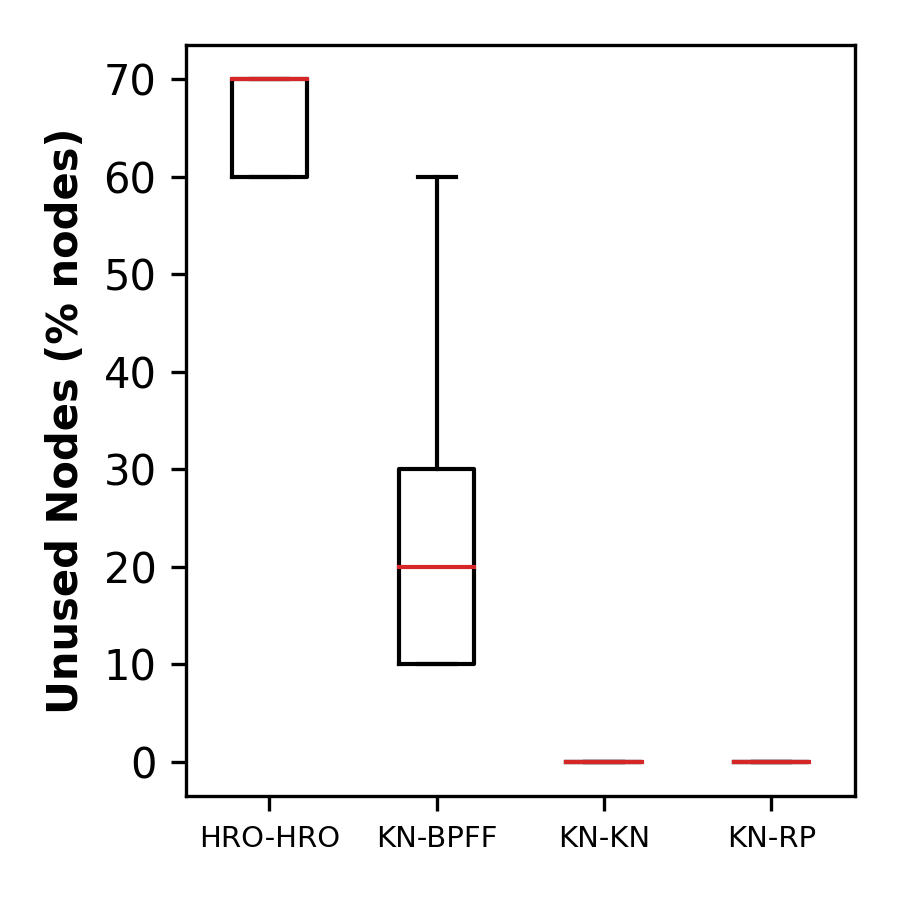
\includegraphics[width=0.3\linewidth]{5_Chapitre3/figures/evaluation/z-nodes-20221212-232143-169224.png}
    }\qquad
    \subfloat[QoS violations (based on tasks with missed deadline)\label{figure:herofake-evaluation-full-penalty}]{
        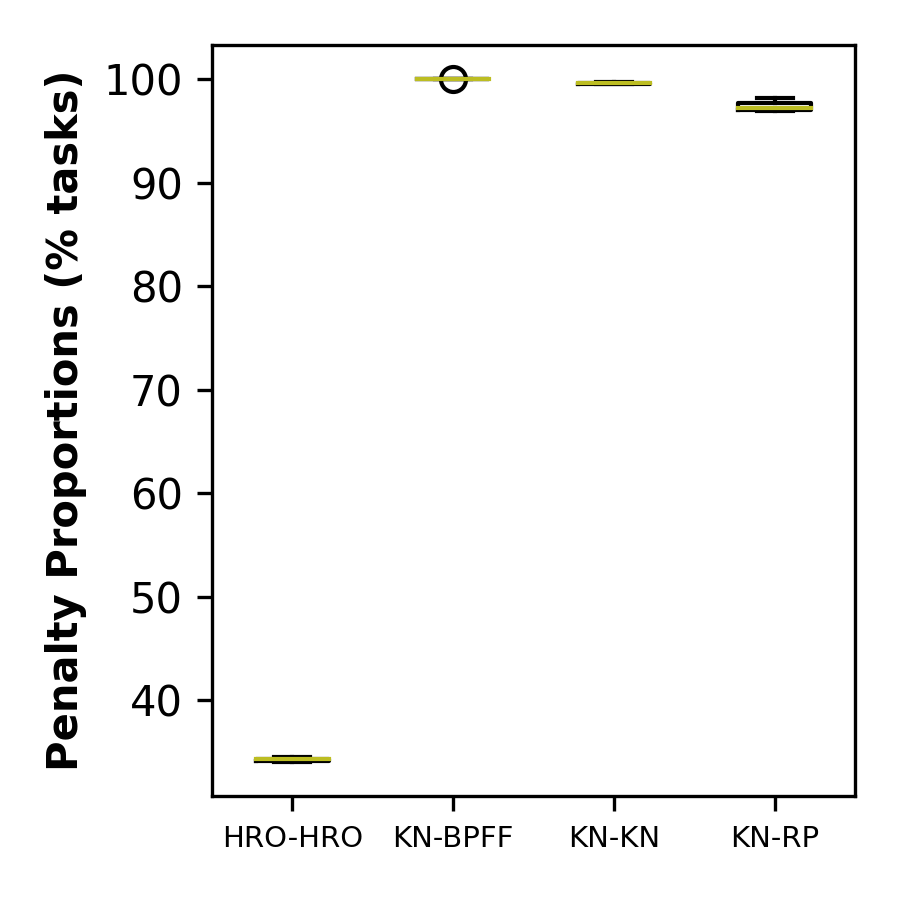
\includegraphics[width=0.3\linewidth]{5_Chapitre3/figures/evaluation/z-penalty-20221212-232143-169224.png}
    }\qquad
    \subfloat[Dynamic energy consumption (in kWh)\label{figure:herofake-evaluation-full-energy}]{
        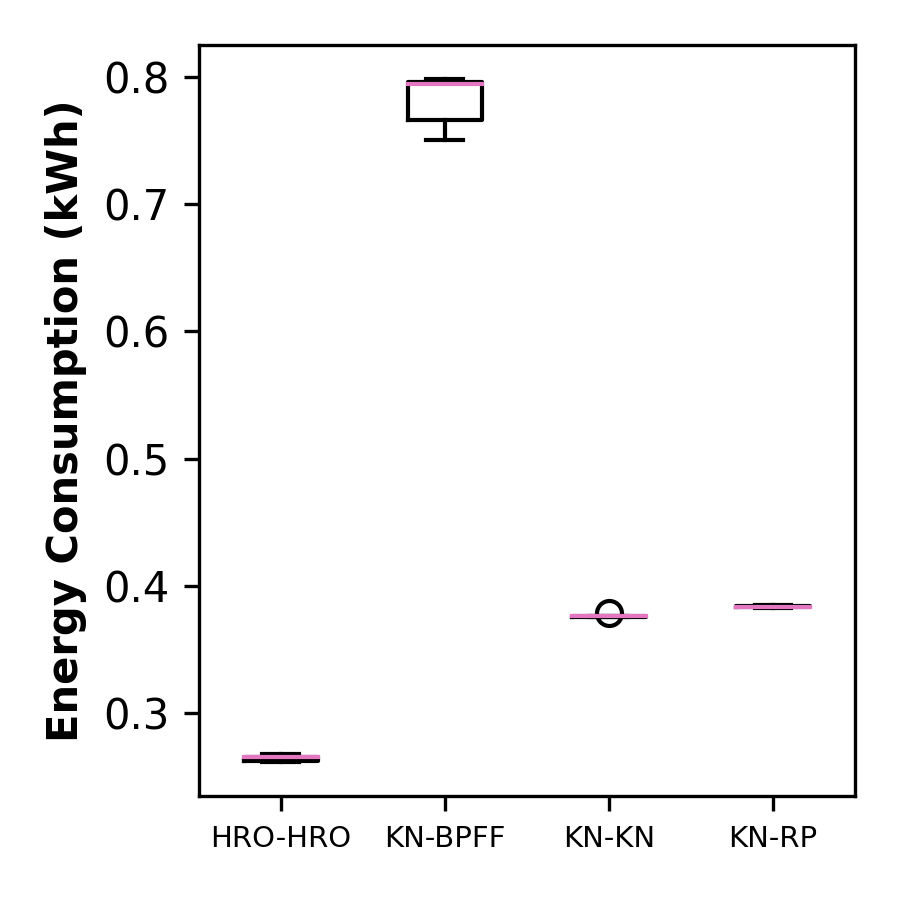
\includegraphics[width=0.3\linewidth]{5_Chapitre3/figures/evaluation/z-energy-20221212-232143-169224.png}
    }
    \caption{Evaluation 1 -- Comparison against baselines}
    \label{figure:herofake-evaluation-hro-full}
\end{figure*}

\begin{figure*}[t]
    \subfloat[Task consolidation (based on the unused node count)\label{figure:herofake-evaluation-mixed-nodes}]{
        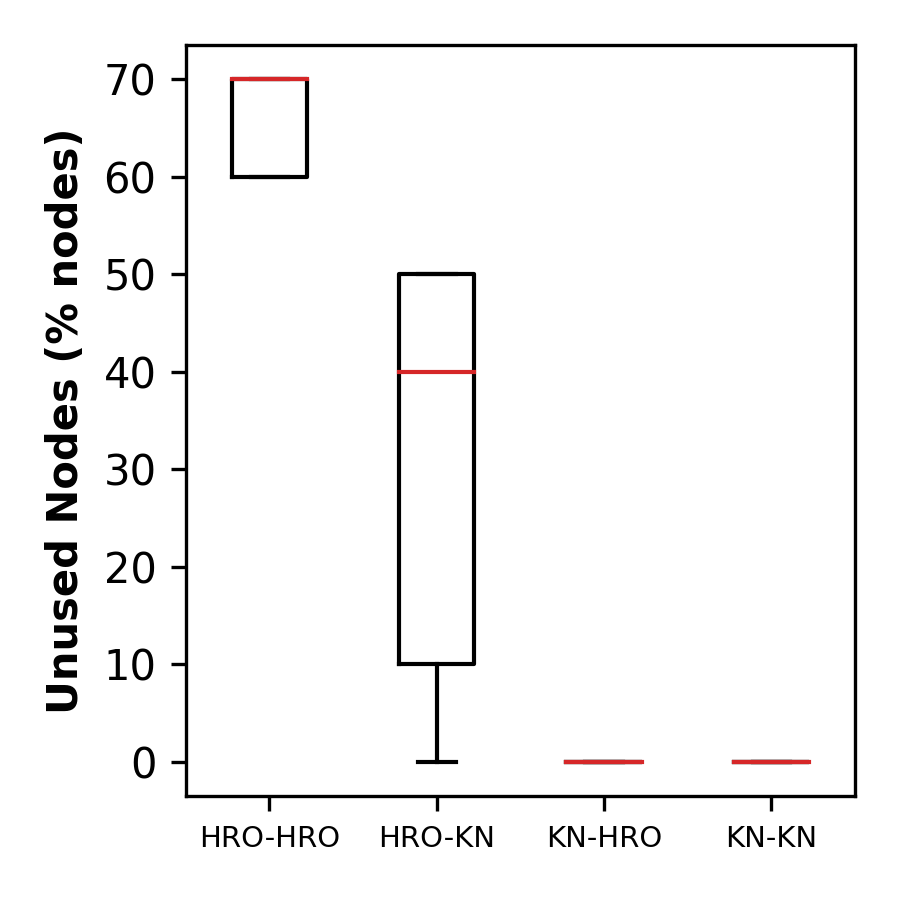
\includegraphics[width=0.3\linewidth]{5_Chapitre3/figures/evaluation/x-nodes-20221212-185844-053283.png}
    }\qquad
    \subfloat[QoS violations (based on tasks with missed deadline)\label{figure:herofake-evaluation-mixed-penalty}]{
        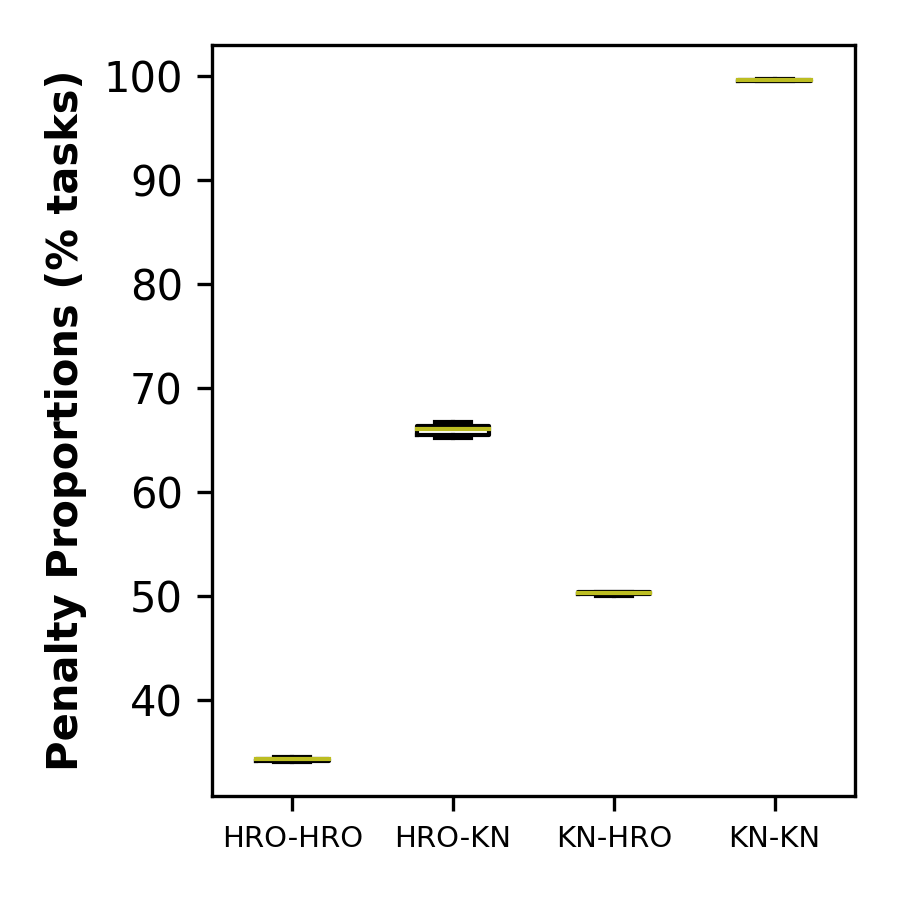
\includegraphics[width=0.3\linewidth]{5_Chapitre3/figures/evaluation/x-penalty-20221212-185844-053283.png}
    }\qquad
    \subfloat[Dynamic energy consumption (in kWh)\label{figure:herofake-evaluation-mixed-energy}]{
        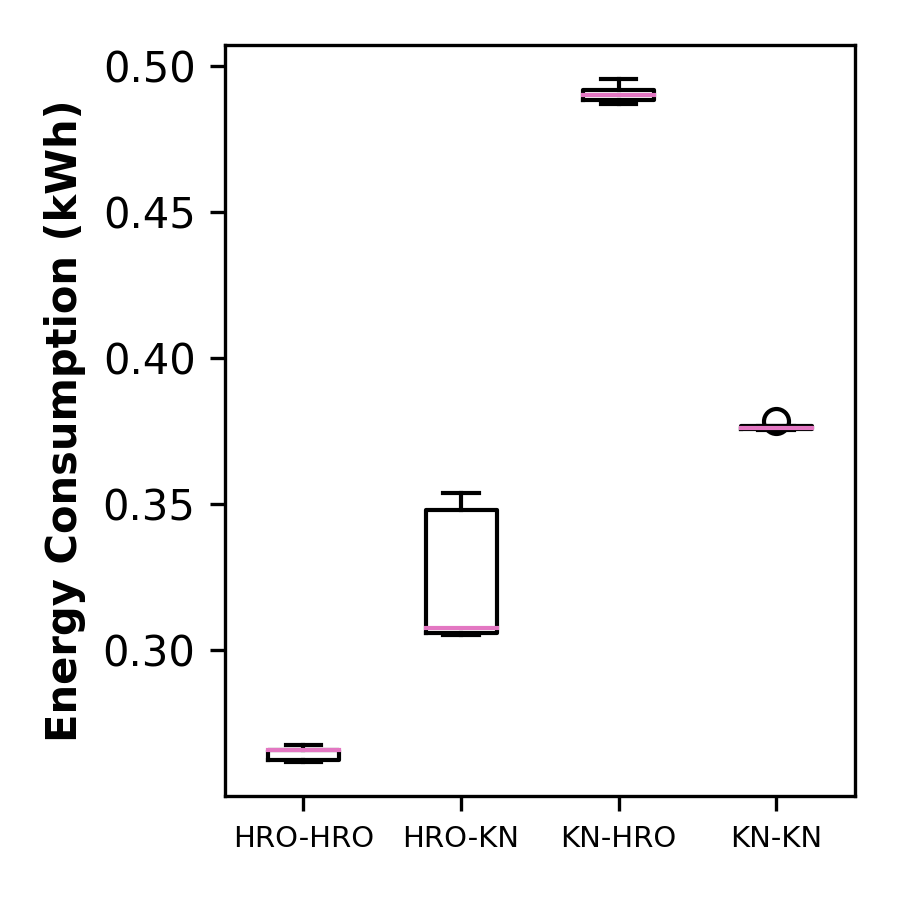
\includegraphics[width=0.3\linewidth]{5_Chapitre3/figures/evaluation/x-energy-20221212-185844-053283.png}
    }
    \caption{Evaluation 2 -- Impact of HeROfake components on the overall performance}
    \label{figure:herofake-evaluation-hro-mixed}
\end{figure*}

\subsection{Experimental setup}

We used measurements from the evaluation of three different machine learning models (see Table~\ref{table:herofake-tasks}). These models have been implemented on three different execution platforms (see Table~\ref{table:herofake-platforms}) as explained in Section~\ref{offline}.

These data served as input for a simulator we built using SimPy~\cite{simpy}. The simulator follows the system model described in sections~\ref{model:nodes}, \ref{model:platforms}, \ref{model:tasks}.

We measured cold start delays for our case study applications, see Table~\ref{table:herofake-tasks}. It appears that execution times are dominated by cold start delays, making adequate resource allocation a stringent requirement to comply with SLAs.

In the performance evaluation part, we compare two autoscalers:
\begin{itemize}
    \item HeROfake (HRO) -- Our heterogeneity-aware, metadata-based resource allocator;
    \item Knative (KN) -- We modeled the Knative autoscaler behavior to the best of our knowledge.
\end{itemize}

Our evaluation extends to four schedulers:

\begin{itemize}
    \item HeROfake (HRO) -- Our cost-aware scheduler that minimizes SLA violations, energy consumption and resource usage;
    \item Knative (KN) -- Knative selects a platform on the most available node~\cite{sureshENSUREEfficientScheduling2020}. Execution platforms are sorted by in-flight requests count. The platform with the shortest queue is selected;
    \item Random Placement (RP) -- Tasks are assigned a random execution platform on a random node;
    %\item Round Robin (RR) -- Load is balanced across nodes by assigning execution platforms to tasks in a cyclic fashion;
    \item Bin Packing First-Fit (BPFF) -- Tasks are consolidated on the minimum number of execution platforms. While a node still has enough memory available for new replicas, it is systematically chosen until it runs out of memory; then, a new node is selected. BPFF is likely to be the scheduling policy for AWS Lambda~\cite{wangPeekingCurtainsServerlessb}.
\end{itemize}

%Note that for each strategy, we still apply some pre-filtering on execution platforms: a task is never assigned a node that could not achieve its execution (i.e. a node that does not meet the task's memory requirements, or that does not provide a suitable execution platform).

We designed a two-step performance evaluation based on simulations:

\begin{itemize}
    \item \textbf{Comparison against baselines} (Figure~\ref{figure:herofake-evaluation-hro-full}): in this part, we compared our HeROfake combination of autoscaler and scheduler (HRO-HRO) to: (1) full-featured Knative autoscaler and scheduler (KN-KN), (2) Knative autoscaler with BPFF scheduler (KN-BPFF), (3) Knative autoscaler with RP scheduler (KN-RP); 
    \item \textbf{Impact of HeROfake components on the overall performance} (Figure~\ref{figure:herofake-evaluation-hro-mixed}): here we discuss the individual impact of each of the autoscaler and the scheduler. To do so, we devised different strategies: (1) using HeROfake autoscaler with Knative scheduler, and (2) using Knative autoscaler with HeROfake scheduler, and we compared those strategies with full featured HeROfake and Knative.
\end{itemize}

The naming of each scenario in these figures consists of two parts divided by a dash symbol. The first part corresponds to the allocation policy; the second part corresponds to the scheduling policy (for example, HRO-KN means we used the HeROfake autoscaler in conjunction with the Knative scheduler). 

%In order to measure the relevance of both our autoscaler and scheduler policies, we proceeded to evaluate them in two configurations. Figure~\ref{figure:herofake-evaluation-hro-full} shows our solution (HRO-HRO) evaluated against vanilla Knative (KN-KN), and Knative autoscaler with baseline schedulers (KN-BPFF, KN-RP). Figure~\ref{figure:herofake-evaluation-hro-mixed} shows our autoscaler and scheduler mixed with Knative's autoscaler and scheduler to evaluate the impact of each component on the overall performances. 

For each of the combinations of autoscaler and scheduler policies, we ran the experiment on a synthetic workload scenario consisting of 50000 tasks (user requests). Tasks are assigned a random type (ResNet50, VGG16 or VGG19) and a random QoS level (high, medium, low) following a uniform distribution, with QoS duration deviations respectively set to 2, 3 and 4. The infrastructure for the scenario consists of 10 nodes (10 CPUs, 6 GPUs, 2 FPGAs).

Weights for the concurrency level (Equation~\ref{eq:herofake-HRO-concurrency-target}) have been set to $k_{ET} = \frac{2}{3}$, $k_{EC} = \frac{1.5}{6}$ and $k_{HP} = \frac{0.5}{6}$. Weights for the scale out decision (Equation~\ref{eq:herofake-HRO-allocation-cost-function}) have been set to $k_{TT} = \frac{2}{3}$, $k_{EC} = \frac{1.5}{6}$ and $k_{HP} = \frac{0.5}{6}$. Weights for the scheduling decision (Equation~\ref{eq:herofake-HRO-scheduling-cost-function}) have been set to $k_{QP} = \frac{2}{3}$, $k_{EC} = \frac{0.5}{6}$ and $k_{TC} = \frac{1.5}{6}$. 

\subsection{Experimental results}

\subsubsection{Comparison against baselines}

\textbf{Tasks consolidation}. Figure~\ref{figure:herofake-evaluation-full-nodes} shows that our combination of autoscaler and scheduler achieves the highest number of unused nodes. Under Knative's autoscaler, the BPFF scheduler ensures the best consolidation, but that policy still needs more than three times the nodes we need with our policy.% We can see that our scheduler comes second best at task consolidation, with almost 70\% of nodes left unused -- a negligible degradation compared to HRO-BPFF.

\textbf{Service Level Agreements}. Figure~\ref{figure:herofake-evaluation-full-penalty} shows that HRO-HRO performs the best in terms of QoS violations, with 35\% of tasks missing their deadlines. This is a huge improvement with regard to the Knative results, where tasks miss their deadlines more than 99\% of the time: the delay introduced by the reactive allocation of resources cannot be compensated in time using only CPUs.

\textbf{Energy consumption}. Figure~\ref{figure:herofake-evaluation-full-energy} shows that our policy, with the HRO autoscaler and scheduler working in conjunction, consistently performs the best in terms of dynamic energy consumption. This is obviously because we allocate hardware accelerators; however, during our evaluation, the makespan for our scenario is similar under Knative and HRO policies (around 13.5 minutes). The BPFF scheduling policy also performs the worst in terms of execution time, as it maximizes the task queues in execution platforms, thus yielding the worst results in terms of energy consumption.

%This is obviously because we allocate hardware accelerators; however, under a BPFF scheduler, our autoscaler shows results barely better than Knative's autoscaler: seeking task consolidation on platforms and nodes seems to yield the worst energy efficiency.

\subsubsection{Impact of each component}

\textbf{Tasks consolidation}. Figure~\ref{figure:herofake-evaluation-mixed-nodes} shows that HRO-HRO performs the best at task consolidation, leaving just under 70\% of the available nodes unused, while Knative's scheduler under our autoscaling policy only achieves 40\% of unused nodes. This result is expected, as Knative's scheduler employs a Least Connected policy. We see mediocre consolidation results for KN-HRO, but for a different reason: this is because our scheduler tries to minimize QoS violations and spreads the task across all the allocated CPUs.

\textbf{Service Level Agreements}. Figure~\ref{figure:herofake-evaluation-mixed-penalty} shows that our scheduler does not perform well in conjunction with Knative's autoscaler. This is because our scheduler tries to minimize penalties: when given only CPUs to work with, it will behave similarly to Knative's scheduler and spread tasks across theses CPUs to limit QoS violations. However, our scheduler under the Knative autoscaler still manages to keep QoS violations at around 50\% of tasks, showing that there is room for improvement even when deploying inference tasks on CPUs only. Note that during our evaluation, the Knative autoscaler gave the worst results regarding cold starts frequency (6.5 more under KN-HRO than under HRO-KN).

\textbf{Energy consumption}. Figure~\ref{figure:herofake-evaluation-mixed-energy} shows that energy consumption is always lower when using our autoscaler, which can allocate hardware accelerators. However, our scheduler used with Knative's autoscaler yields the worst results in terms of energy consumption. This is again the result of the scheduler trying to minimize penalties and spreading task across a maximum number of CPUs.

\section{State of the Art} \label{section:herofake-sota}

Previous work focused on autoscaling platforms for the deployment of short-lived tasks, comprised in applications exhibiting unpredictable load patterns. Table~\ref{table:herofake-sota} summarises how these contributions differ from our target platform.

%Gujarati et al.~\cite{gujaratiSwayamDistributedAutoscaling2017} propose a distributed framework for allocating and scaling resources to support on-demand inference workloads, while meeting SLA on incoming requests and decreasing resource utilization. Ling et al.~\cite{lingPigeonDynamicEfficient2019} propose a function-level scheduler for Kubernetes that allows running short-lived functions using a pool of pre-warmed containers, mapping each FaaS service to suitable containers according to its hardware resources requirements. Zhang et al.~\cite{zhangMArkExploitingCloud} propose a hybrid autoscaling mechanism that opportunistically uses serverless instances to cover sudden spikes in load, while relying on a pool of reserved GPU-enabled AWS VMs for the majority of inference tasks, in order to achieve reduced operation costs and achieve SLO. Suresh et al.~\cite{sureshENSUREEfficientScheduling2020} propose a function-level scheduler that caterogizes tasks between interactive, short-lived, event-triggered tasks, and massively parallel, batch, back-end tasks, with the objective to decrease resource usage and provide acceptable latency guarantees. Mampage et al.~\cite{mampageDeadlineawareDynamicResource2021} propose a function placement and resource management policy that targets reduced resource consumption while meeting users' applications deadlines. Singhvi et al.~\cite{singhviAtollScalableLowLatency2021} propose parting with reactive sandbox allocation and instead proactively provisioning nodes so as to meet user-defined function deadlines. Yang et al.~\cite{yangINFlessNativeServerless2022} propose a serverless platform aimed at deploying and scaling inference tasks under user-defined SLOs, with low-latency, high-throughput constraints. Cho et al.~\cite{choSLADrivenMLInference} propose a serverless scheduler that takes into account heterogeneity in the infrastructure and in the users' requests to achieve SLAs (target latency, inference per second) and optimize for resource usage.

Some of these contributions attempted to achieve SLA with unreserved resources~\cite{gujaratiSwayamDistributedAutoscaling2017, zhangMArkExploitingCloud, mampageDeadlineawareDynamicResource2021, singhviAtollScalableLowLatency2021, handaoui2020releaser, handaoui2020salamander, yalles2022riscless}.
Among these contributions, some focus on the use of additional heterogeneous hardware resources to accelerate workload execution~\cite{zhangMArkExploitingCloud, lingPigeonDynamicEfficient2019, yangINFlessNativeServerless2022}.
They often require overprovisioning resources to make use of hardware acceleration, e.g. by relying on reserved AWS instances that provide access to GPUs~\cite{zhangMArkExploitingCloud}, using a pool of pre-warmed containers~\cite{lingPigeonDynamicEfficient2019}, or even proactively provisioning nodes to meet user-defined function deadlines~\cite{singhviAtollScalableLowLatency2021}. These interesting solutions however may fall short in terms of resource usage and would incur additional energy consumption in a private cloud.

Furthermore, some authors focus on homogeneous infrastructures \cite{gujaratiSwayamDistributedAutoscaling2017, sureshENSUREEfficientScheduling2020, mampageDeadlineawareDynamicResource2021, singhviAtollScalableLowLatency2021, yangINFlessNativeServerless2022}. Those studies could hardly fit the private cloud setting we target, where resources are usually transient and heterogeneous. Also, some of these contributions propose task models that do not cover user-defined, per-request SLA~\cite{sureshENSUREEfficientScheduling2020, lingPigeonDynamicEfficient2019}. Finally, some of these contributions are performance-oriented rather than cost-oriented which is crucial in our cloud context~\cite{gujaratiSwayamDistributedAutoscaling2017, lingPigeonDynamicEfficient2019, singhviAtollScalableLowLatency2021, choSLADrivenMLInference}.

In spite of power being one of the topmost part of the total cost of ownership (TCO) in a datacenter -- sometimes exceeding the cost of buying hardware~\cite{7279063} -- to the best of our knowledge, none of these contributions cover the impact of dynamic allocation and dynamic placement on energy consumption, nor do they consider energy consumption as a QoS metric. This is a serious limitation, as optimizing for task consolidation opens possibilities for throttling and powering-off policies that can have a major impact on a datacenter's energy efficiency~\cite{chaurasiaComprehensiveSurveyEnergyaware2021}.

\section{Conclusion and Future Work}

In this paper, we introduced HeROfake, our framework for the deployment of short-lived, interactive deepfake detection tasks on a private, heterogeneous serverless cloud.

We presented the two phases that make up this framework: an offline phase during which we characterize execution platform performances and task requirements; and an online phase during which we dynamically allocate resources and schedule tasks to run on those platforms.

Experimental results show that while total task execution time in HeROfake is similar to vanilla Knative, we achieve more than 60\% reduction in QoS penalties; tasks are consolidated on less than 40\% of the infrastructure's nodes, with 77\% execution platforms left unused; and dynamic energy consumption is reduced by 35\% as compared to Knative.

The inclusion of video handling in the framework is an interesting challenge, as it would introduce dependencies between tasks. Function executions would not be \textit{stateless} anymore, resulting in the necessity to tackle the problem of intermediate data storage in a serverless infrastructure.%M since function state has to be persisted in disaggregated storage, applications can suffer from the shipping time of data to compute nodes \cite{mullerLambadaInteractiveData2020}.

%This perspective can be linked to the introduction of heterogeneity in user requests. Input data size and locality could vary a lot between pictures and videos, and open possibilities of batching requests to study the impact on the performances of our platform.

We also intend to extend the simulator with a parser so as to be able to use real datacenter traces as input scenarios, instead of using synthetic workloads only. %This could give us the opportunity to learn from these traces and apply machine learning algorithms in the workload characterization phase, allowing us to generalize our framework to arbitrary applications without generating \textit{a priori} metadata on tasks.
